\documentclass[10pt,aspectratio=169]{beamer}

\usetheme{metropolis}
\usepackage[utf8]{inputenc}
\usepackage[T1]{fontenc}
\usepackage[french]{babel}
\usepackage{graphicx}
\usepackage{booktabs}
\usepackage{array}
\usepackage{amsmath}
\usepackage{xcolor}

\graphicspath{{figures/}}

\title{OceanLens -- Ordre des expériences FM}
\subtitle{De v4 aux fine-tunings de v4\_s1}
\author{El-Mehdi Boulaalam}
\date{\today}

\newcommand{\smallnote}[1]{\vspace{0.3em}{\scriptsize\textcolor{gray}{#1}}}
\newcommand{\good}{\textcolor{green!50!black}{\textbf{+}}}
\newcommand{\bad}{\textcolor{red!70!black}{\textbf{--}}}

\begin{document}

\maketitle

\begin{frame}{Message principal}
\begin{itemize}
  \item On a exploré deux familles de modifications: \textbf{architecture/training} puis \textbf{inférence/fine-tuning}.
  \item La meilleure base expérimentale est devenue \textbf{v4\_s1\_logit\_t}: même pipeline CNO+FM, mais un meilleur choix de sampling temporel.
  \item Les erreurs restantes ne viennent pas seulement du solveur: elles révèlent aussi un problème de \textbf{variance}, de \textbf{conditionnement trop fort}, et de \textbf{distribution régionale}.
\end{itemize}
\end{frame}

\begin{frame}{Pipeline commun à toutes les expériences}
\begin{columns}[T,onlytextwidth]
\column{0.55\textwidth}
\begin{enumerate}
  \item Entrée LR normalisée: $\mu_{\mathrm{LR}}$ avec 5 variables.
  \item CNO prédit une correction déterministe: $\mu = \mathrm{LR} + \mathrm{CNO}(\mathrm{LR})$.
  \item FM apprend le résidu HR autour de $\mu$.
  \item Pendant le training:
  \[
    x_t = (1-t)x_0 + tx_1,\quad v^* = x_1 - x_0
  \]
  \item Le U-Net prédit $v_\theta(x_t,t,\mathrm{condition})$.
\end{enumerate}
\column{0.42\textwidth}
\textbf{Mots-clés}
\begin{itemize}
  \item $x_0$: bruit gaussien.
  \item $x_1$: cible résiduelle HR -- $\mu$.
  \item $t$: temps du chemin FM.
  \item condition: $\mu$, LR, masque, variantes selon config.
  \item loss principale: MSE sur la vitesse.
\end{itemize}
\end{columns}
\end{frame}

\begin{frame}{Ordre des expériences}
\begin{table}
\scriptsize
\begin{tabular}{p{0.16\linewidth}p{0.32\linewidth}p{0.29\linewidth}p{0.15\linewidth}}
\toprule
\textbf{Version} & \textbf{Ce qu'on change} & \textbf{Pourquoi} & \textbf{Inspiration} \\
\midrule
v4 & baseline CNO+FM conditionnel & Point de départ propre & Flow Matching standard \\
v4\_s1 & logit-normal $t$ & Plus de poids aux temps intermédiaires utiles & Diffusion/FM training tricks \\
v4\_s2 & coupling indépendant & Tester si OT/minibatch-OT aide vraiment & Conditional FM / OT coupling \\
v4\_s3 & no attention & Tester le rôle de l'attention bottleneck & Ablation architecture U-Net \\
v4\_s4 & condition avec gradient de $\mu$ & Donner les fronts explicitement au FM & CorrDiff / downscaling guidé gradients \\
v5 & FM-only / autre référence & Voir si CNO est indispensable & Generative residual baseline \\
\bottomrule
\end{tabular}
\end{table}
\end{frame}

\begin{frame}{Baseline v4: rôle dans la campagne}
\begin{columns}[T,onlytextwidth]
\column{0.52\textwidth}
\begin{itemize}
  \item \textbf{Objectif}: valider le pipeline complet CNO + FM.
  \item \textbf{Conditionnement}: le FM part d'une solution déterministe $\mu$ déjà très informative.
  \item \textbf{Observation}: les grandes structures sont cohérentes, mais les résidus FM peuvent rester trop faibles.
  \item \textbf{Interprétation}: le modèle apprend souvent une correction prudente autour du CNO.
\end{itemize}
\column{0.44\textwidth}
\centering
\includegraphics[width=\linewidth,height=0.54\textheight,keepaspectratio]{01_all_variants.png}
\smallnote{Comparaison des résidus thetao, day 0.}
\end{columns}
\end{frame}

\begin{frame}{v4\_s1\_logit\_t: le meilleur point de départ}
\begin{columns}[T,onlytextwidth]
\column{0.48\textwidth}
\textbf{Changement}
\begin{itemize}
  \item On ne tire plus $t$ uniformément.
  \item On utilise un sampling de type \textbf{logit-normal}.
  \item Effet: plus de samples là où la trajectoire est la plus informative.
\end{itemize}
\textbf{Pourquoi}
\begin{itemize}
  \item Le modèle voit mieux les états intermédiaires difficiles.
  \item La trajectoire FM est moins dominée par les extrêmes faciles $t\approx0$ ou $t\approx1$.
\end{itemize}
\column{0.48\textwidth}
\centering
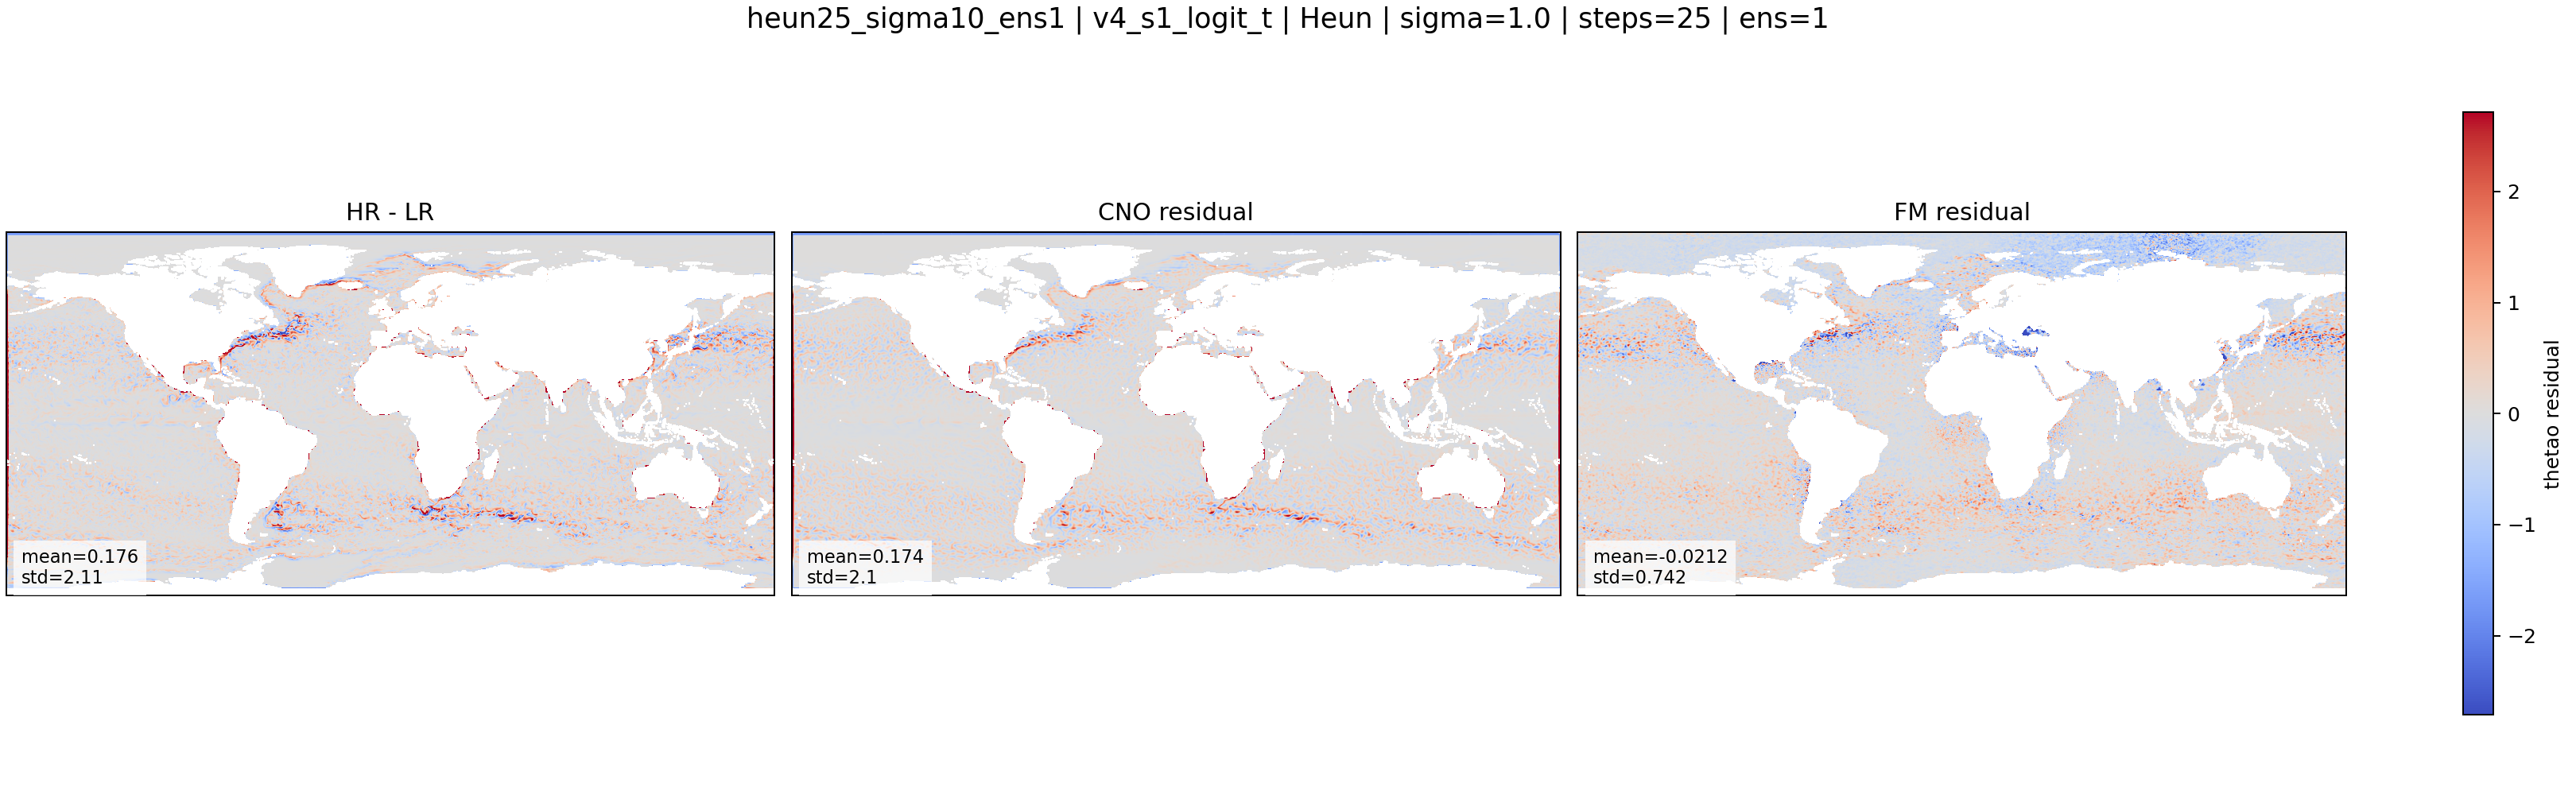
\includegraphics[width=\linewidth]{02_s1_heun25_sigma10_ens1.png}
\smallnote{v4\_s1, Heun 25, $\sigma=1.0$, ensemble 1.}
\end{columns}
\end{frame}

\begin{frame}{v4\_s2, v4\_s3, v4\_s4: ablations}
\begin{table}
\scriptsize
\begin{tabular}{p{0.17\linewidth}p{0.31\linewidth}p{0.39\linewidth}}
\toprule
\textbf{Version} & \textbf{Modification} & \textbf{Lecture expérimentale} \\
\midrule
v4\_s2 & Coupling indépendant / minibatch-OT différent & Teste si l'appariement bruit-cible change la variance et la structure. \\
v4\_s3 & Attention retirée au bottleneck & Si les grandes structures se dégradent, l'attention portait du contexte global. \\
v4\_s4 & Ajout de gradients de $\mu$ dans la condition & Donne explicitement les fronts; utile pour courants, upwellings, côtes. \\
v5 & Référence FM-only & Sert à mesurer ce qu'on perd sans le fort prior CNO. \\
\bottomrule
\end{tabular}
\end{table}

\vspace{0.5em}
\textbf{Conclusion pratique}: v4\_s1 est restée la base la plus saine pour les tests suivants.
\end{frame}

\begin{frame}{Résultat global des variantes v4}
\centering
\includegraphics[width=0.96\linewidth,height=0.76\textheight,keepaspectratio]{01_all_variants.png}
\smallnote{Lecture: comparer HR-LR, résidu CNO, résidu FM et artefacts régionaux.}
\end{frame}

\begin{frame}{Pourquoi tester le solveur à l'inférence ?}
\begin{columns}[T,onlytextwidth]
\column{0.48\textwidth}
\textbf{Hypothèse}
\begin{itemize}
  \item Euler 20 peut être trop grossier pour intégrer la trajectoire FM.
  \item Heun est un solveur d'ordre 2: deux évaluations du réseau par pas.
  \item Il réduit l'erreur numérique sans changer le training.
\end{itemize}
\textbf{Inspiré de}
\begin{itemize}
  \item pratiques CorrDiff / AFM;
  \item littérature FM météo/downscaling;
  \item comparaison NFE qualité/coût.
\end{itemize}
\column{0.48\textwidth}
\centering
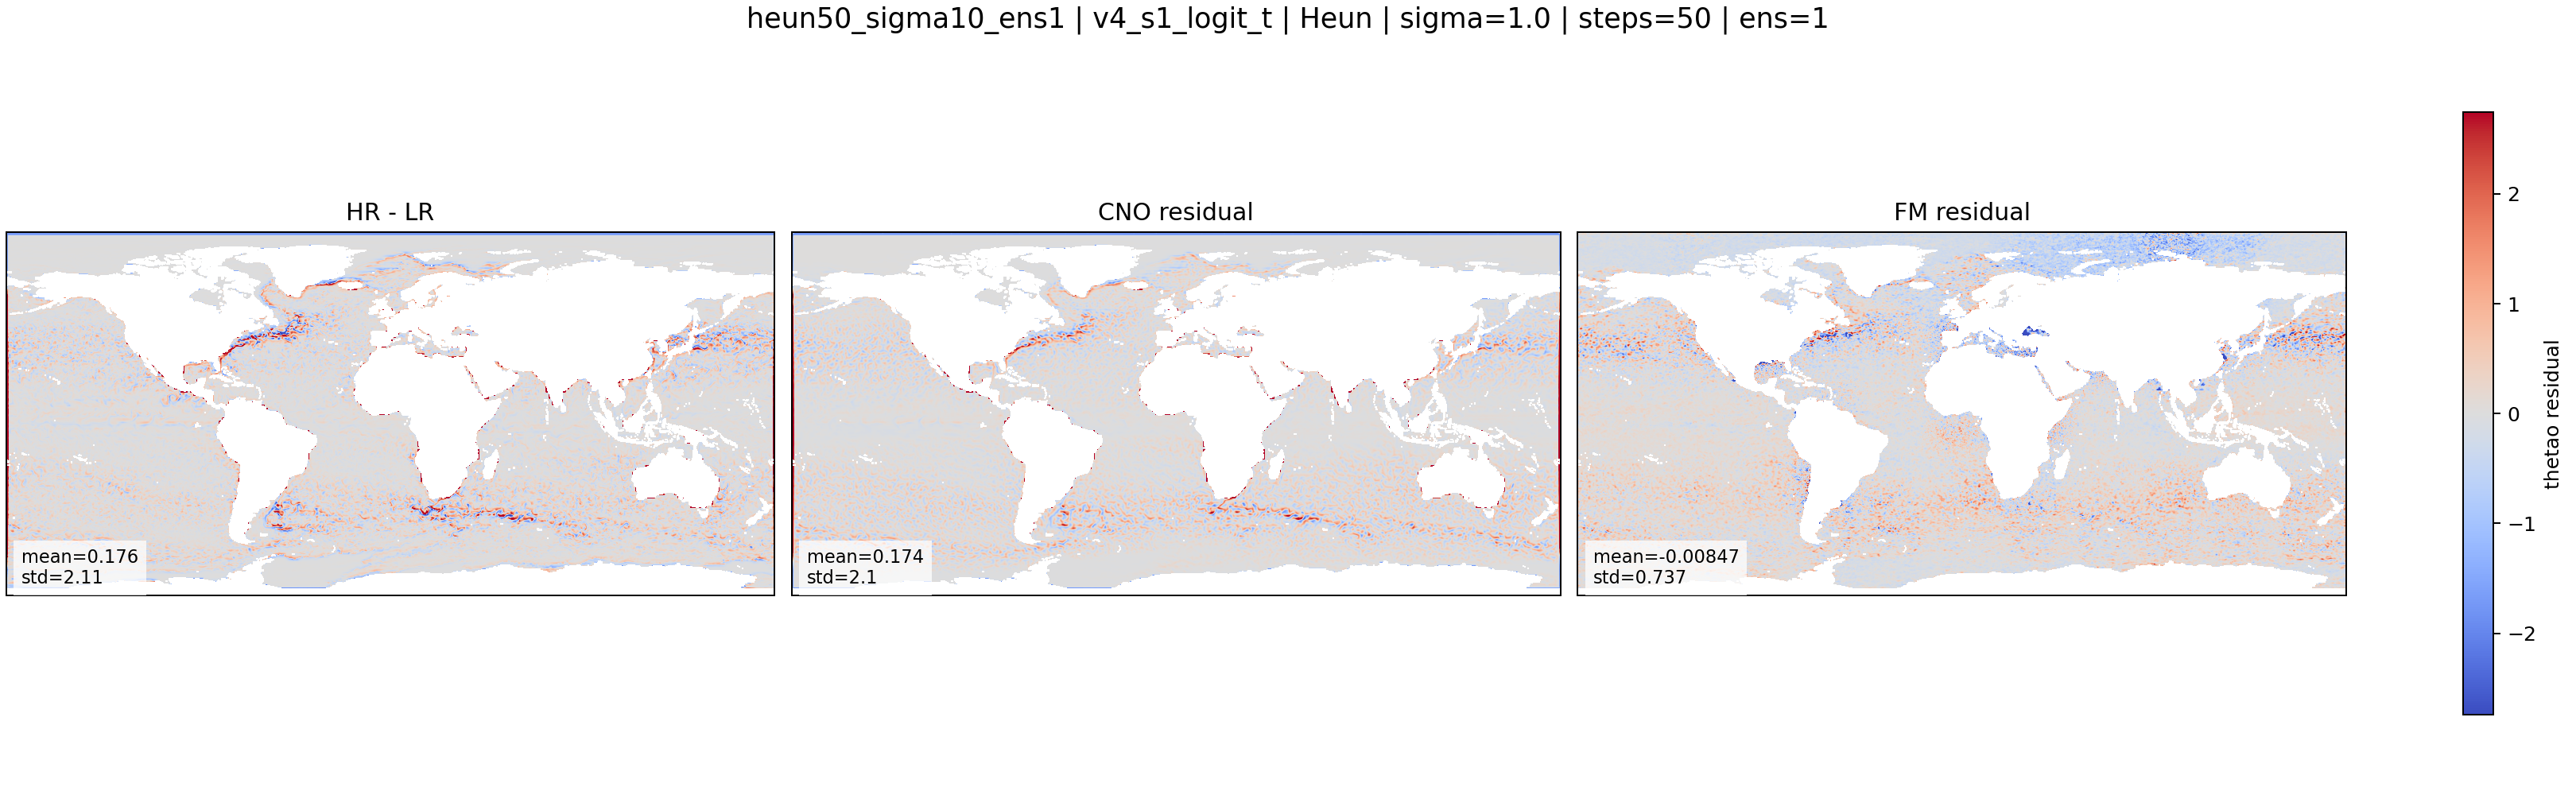
\includegraphics[width=\linewidth]{03_s1_heun50_sigma10_ens1.png}
\smallnote{v4\_s1, Heun 50, $\sigma=1.0$, ensemble 1.}
\end{columns}
\end{frame}

\begin{frame}{Ablation solveur: Heun 25 vs Heun 50}
\begin{columns}[T,onlytextwidth]
\column{0.49\textwidth}
\centering
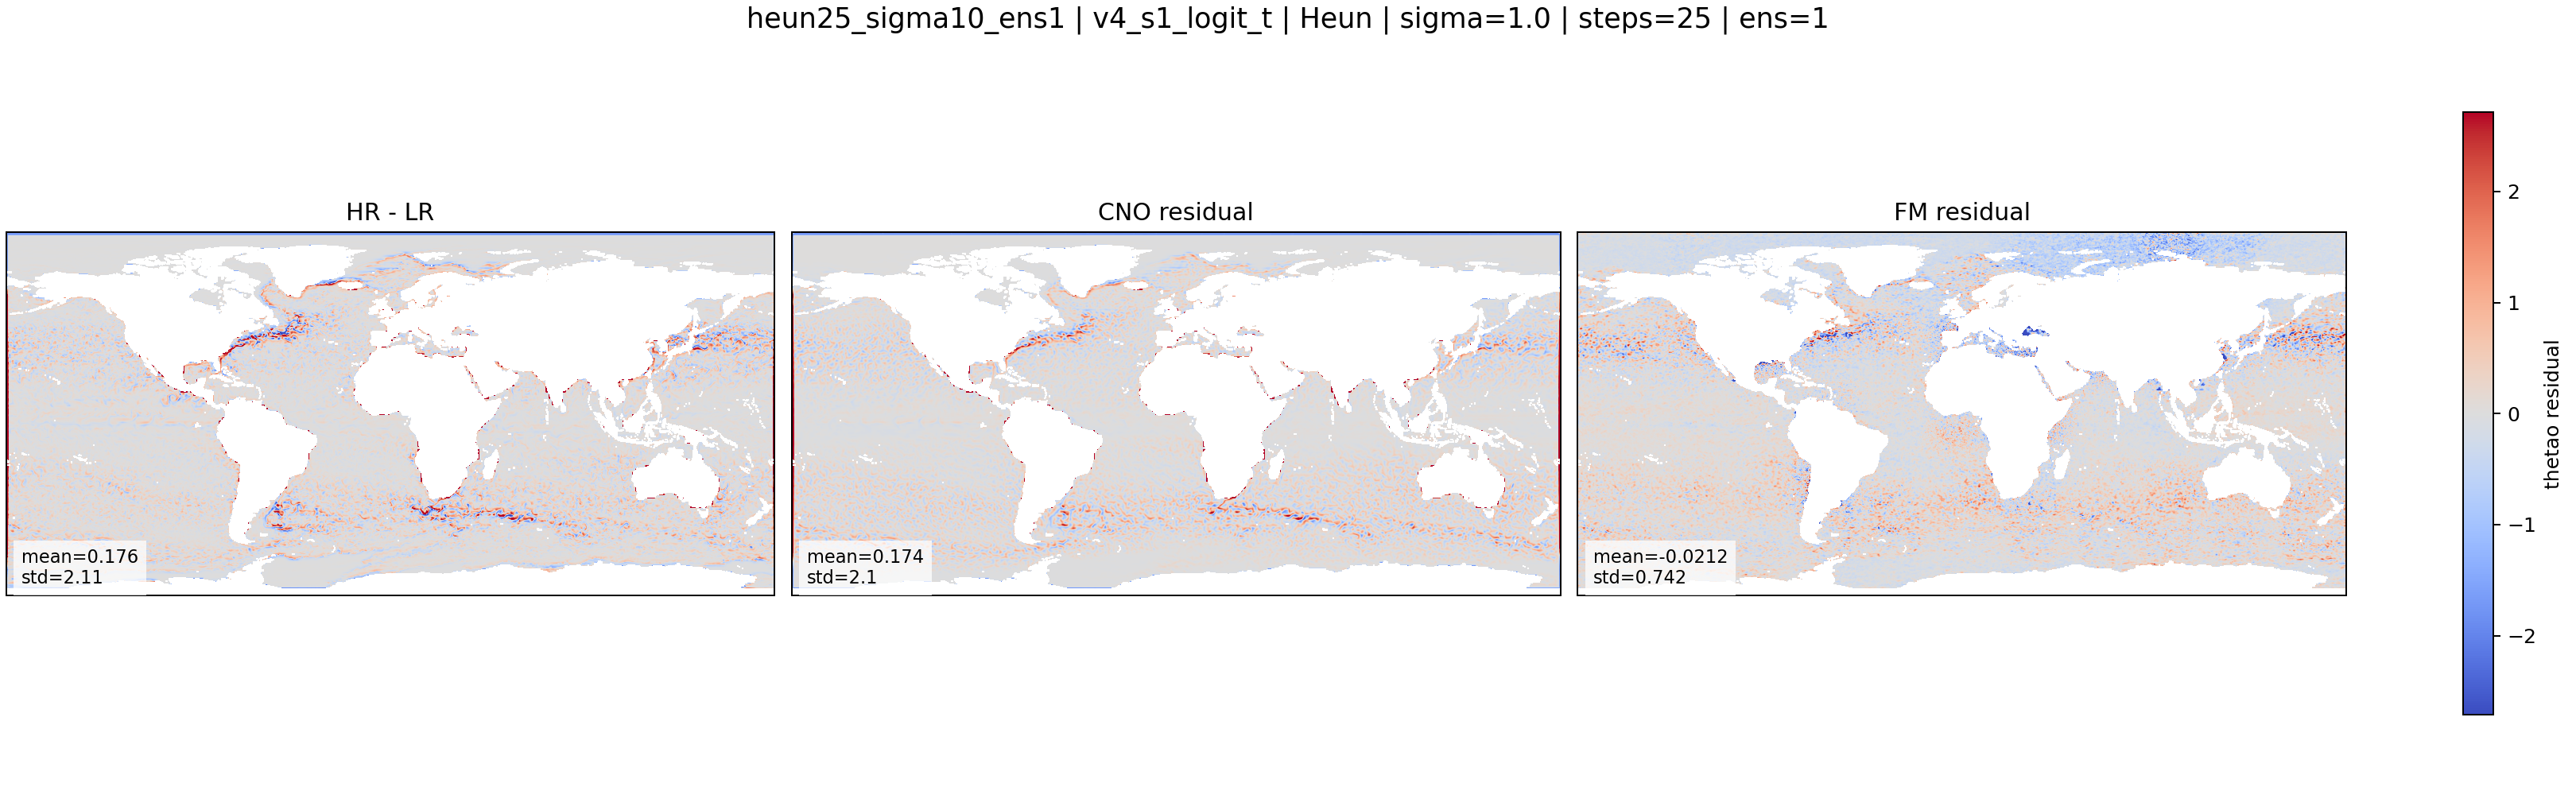
\includegraphics[width=\linewidth]{02_s1_heun25_sigma10_ens1.png}
\smallnote{Heun 25, $\sigma=1.0$, ens=1.}
\column{0.49\textwidth}
\centering
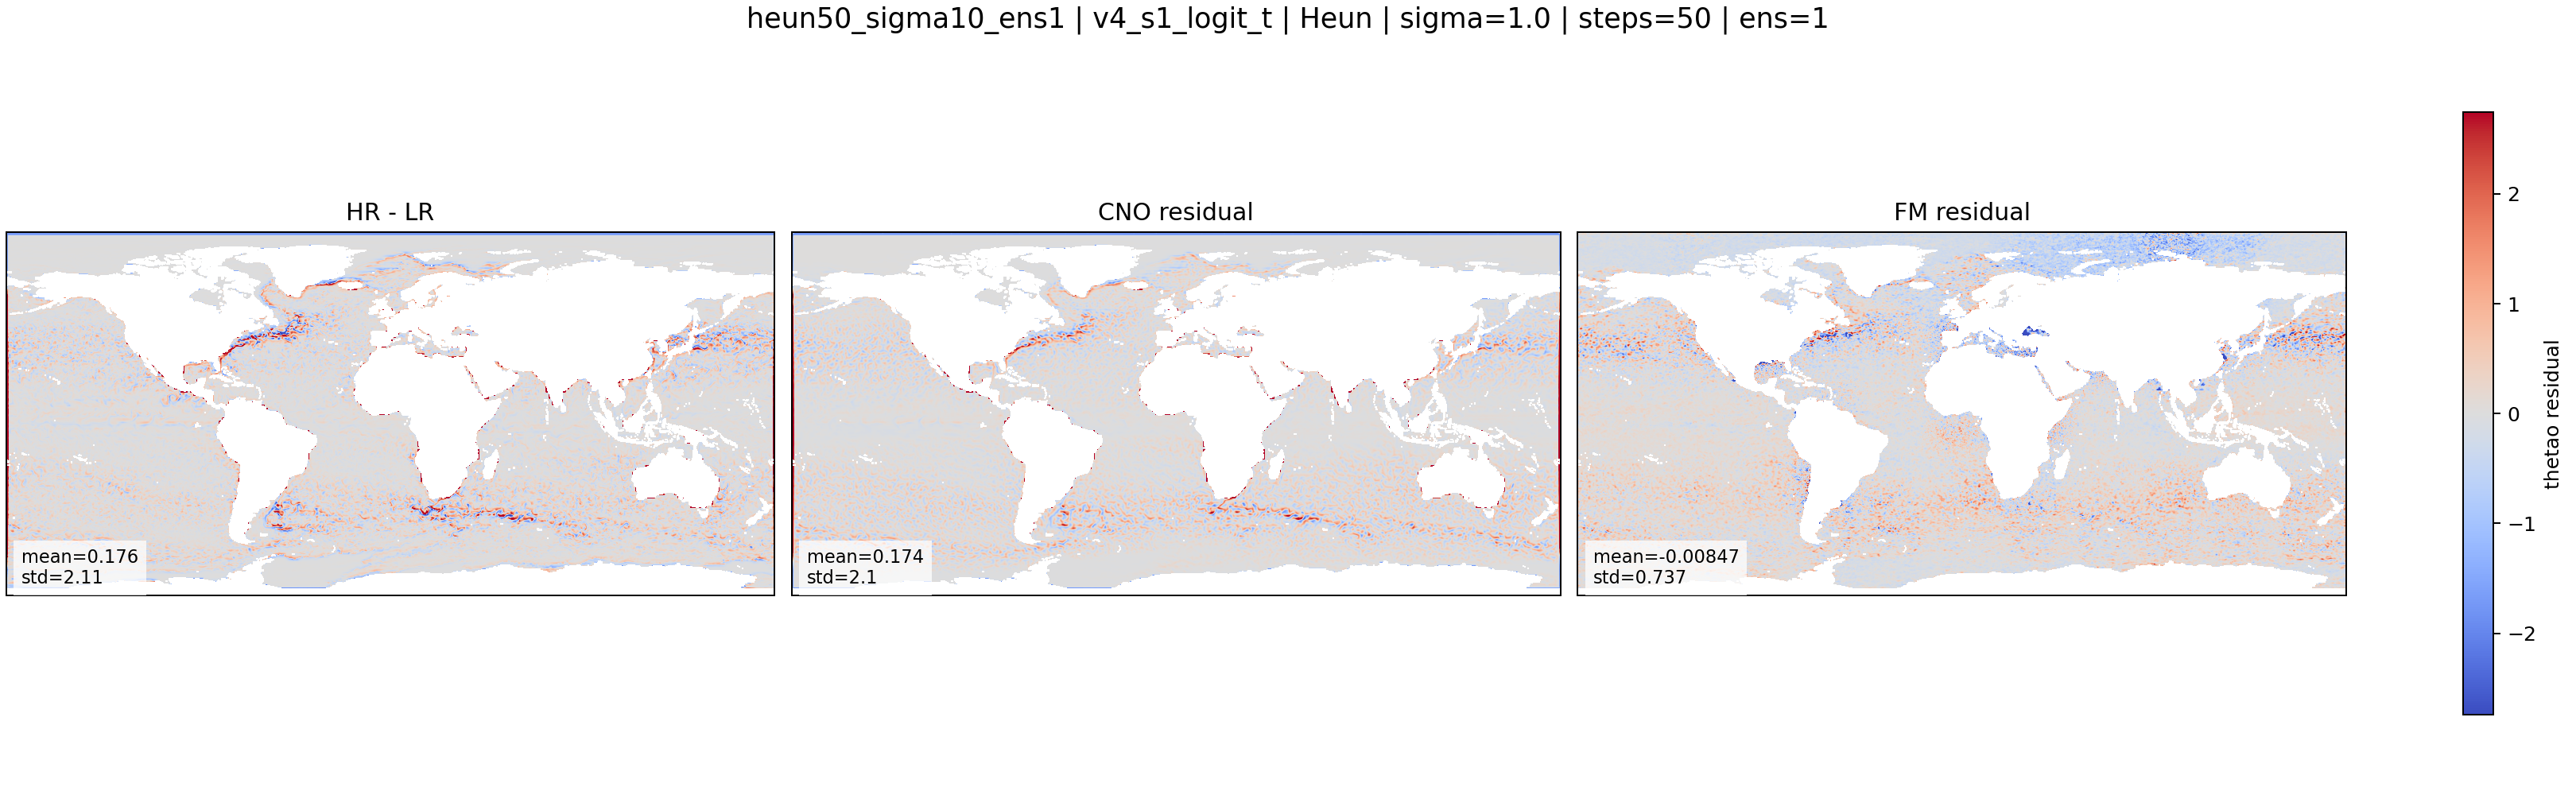
\includegraphics[width=\linewidth]{03_s1_heun50_sigma10_ens1.png}
\smallnote{Heun 50, $\sigma=1.0$, ens=1.}
\end{columns}

\vspace{0.4em}
\textbf{Interprétation}: augmenter les pas stabilise l'intégration, mais ne suffit pas à résoudre entièrement la sous-dispersion.
\end{frame}

\begin{frame}{Ablation bruit initial: $\sigma=1.1$ et $\sigma=1.2$}
\begin{columns}[T,onlytextwidth]
\column{0.49\textwidth}
\centering
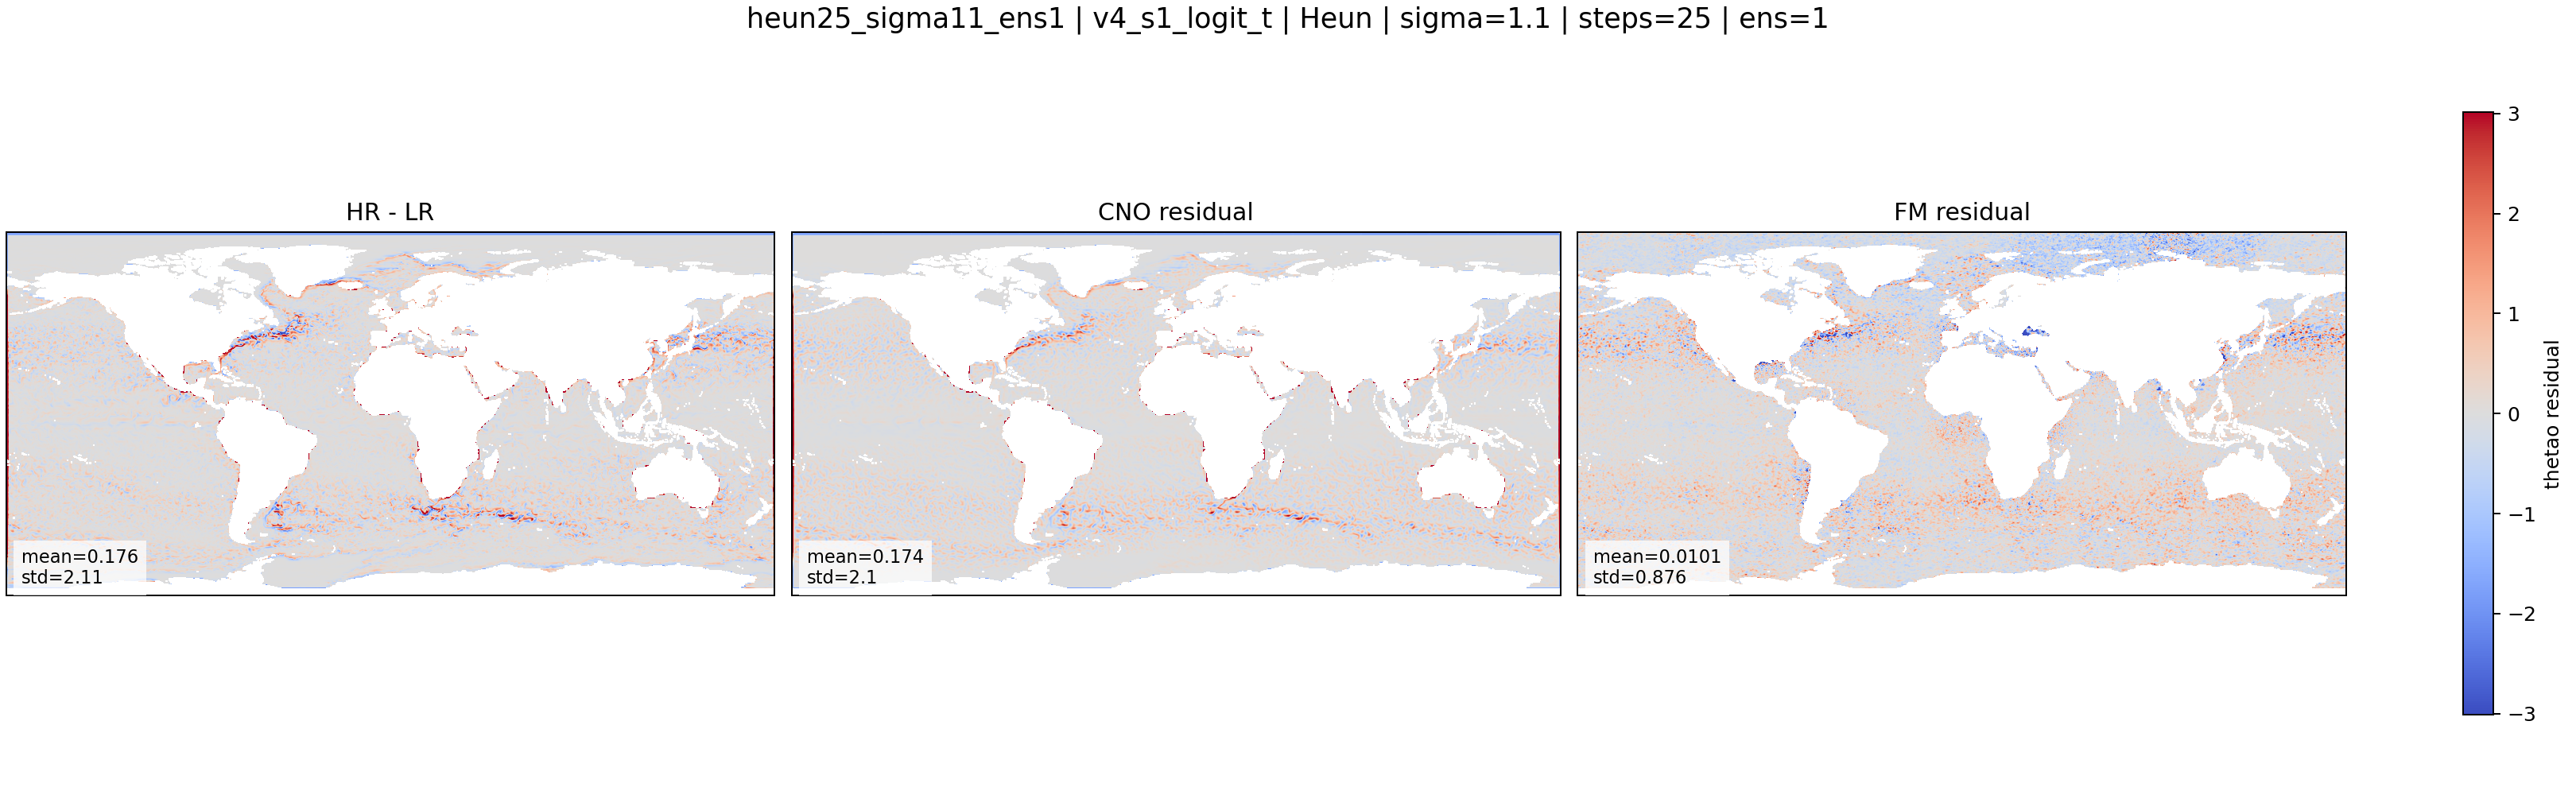
\includegraphics[width=\linewidth]{05_s1_heun25_sigma11_ens1.png}
\smallnote{Heun 25, $\sigma=1.1$, ens=1.}
\column{0.49\textwidth}
\centering
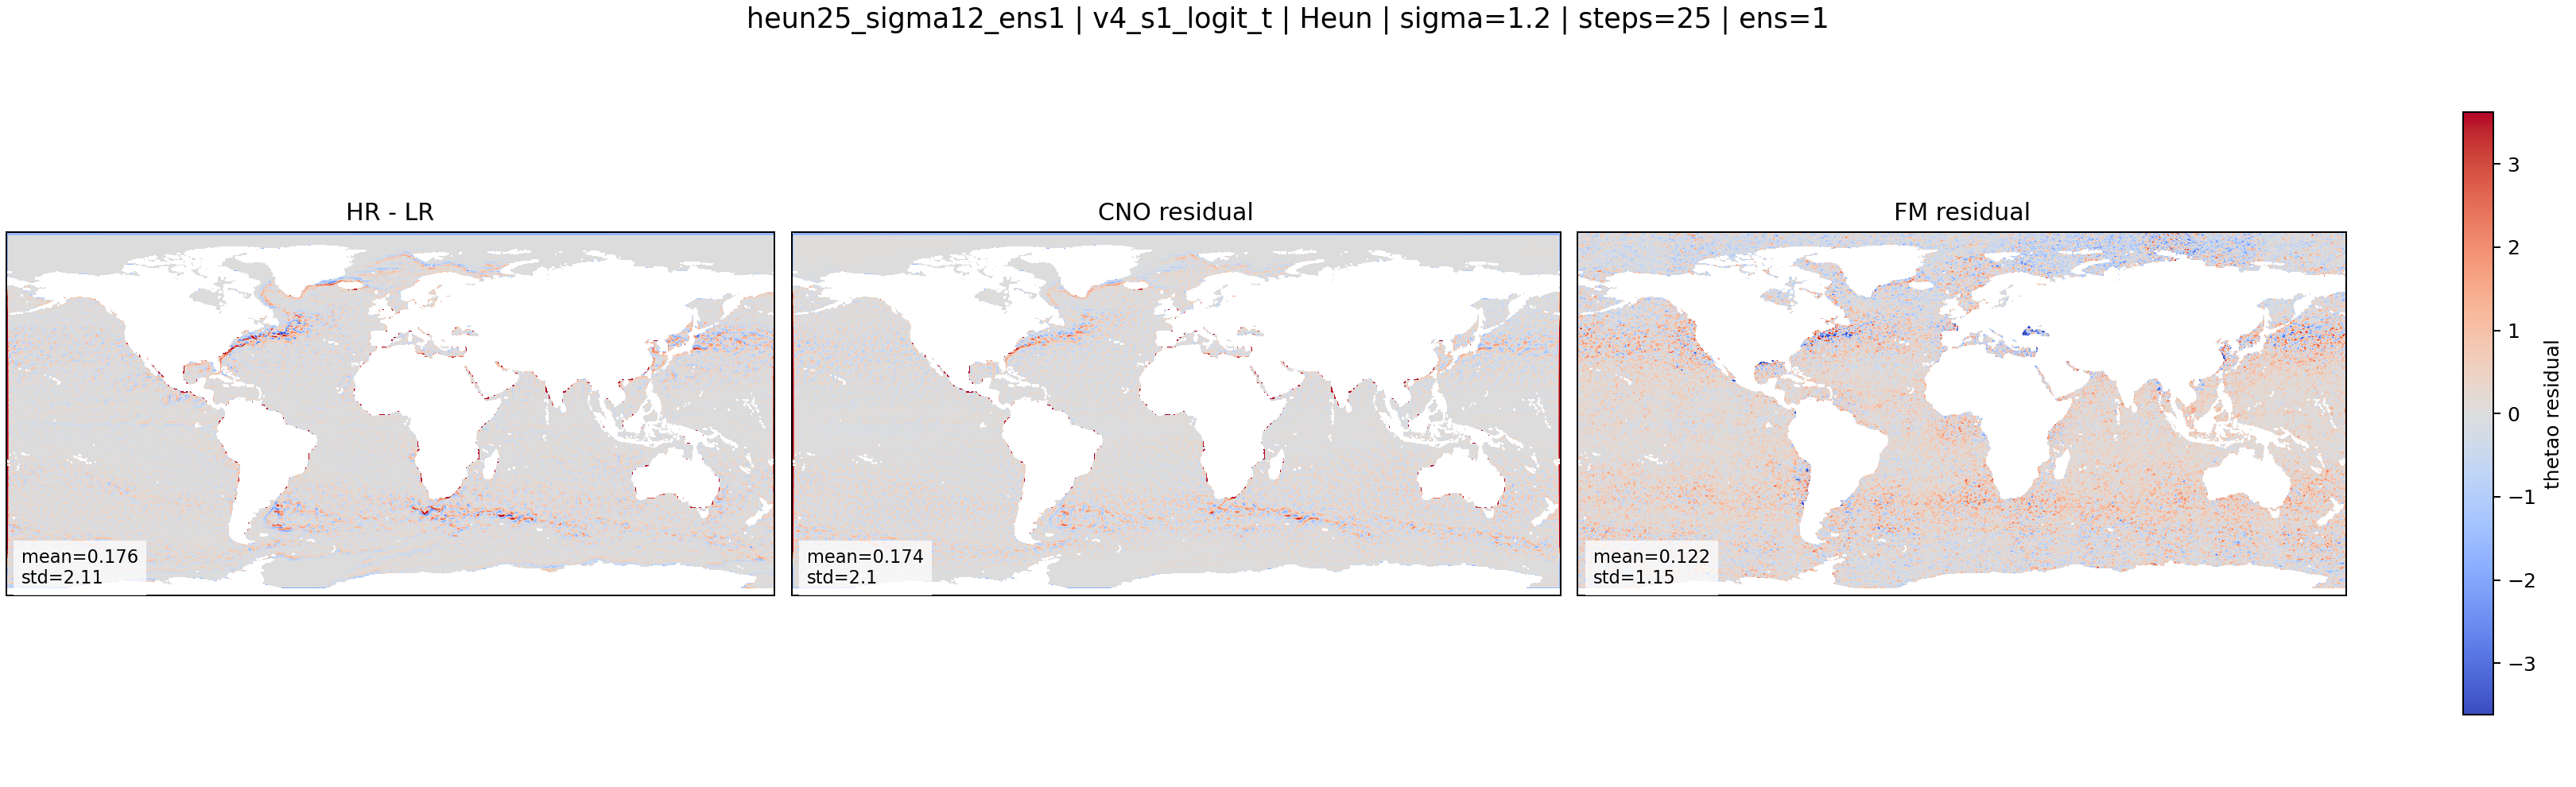
\includegraphics[width=\linewidth]{06_s1_heun25_sigma12_ens1.png}
\smallnote{Heun 25, $\sigma=1.2$, ens=1.}
\end{columns}

\vspace{0.4em}
\textbf{Interprétation}: $\sigma$ augmente l'énergie du bruit initial. Trop haut, il peut réveiller des hautes fréquences mais aussi amplifier des artefacts.
\end{frame}

\begin{frame}{Ensemble: pourquoi ens=32 n'est pas automatiquement meilleur visuellement}
\begin{columns}[T,onlytextwidth]
\column{0.49\textwidth}
\centering
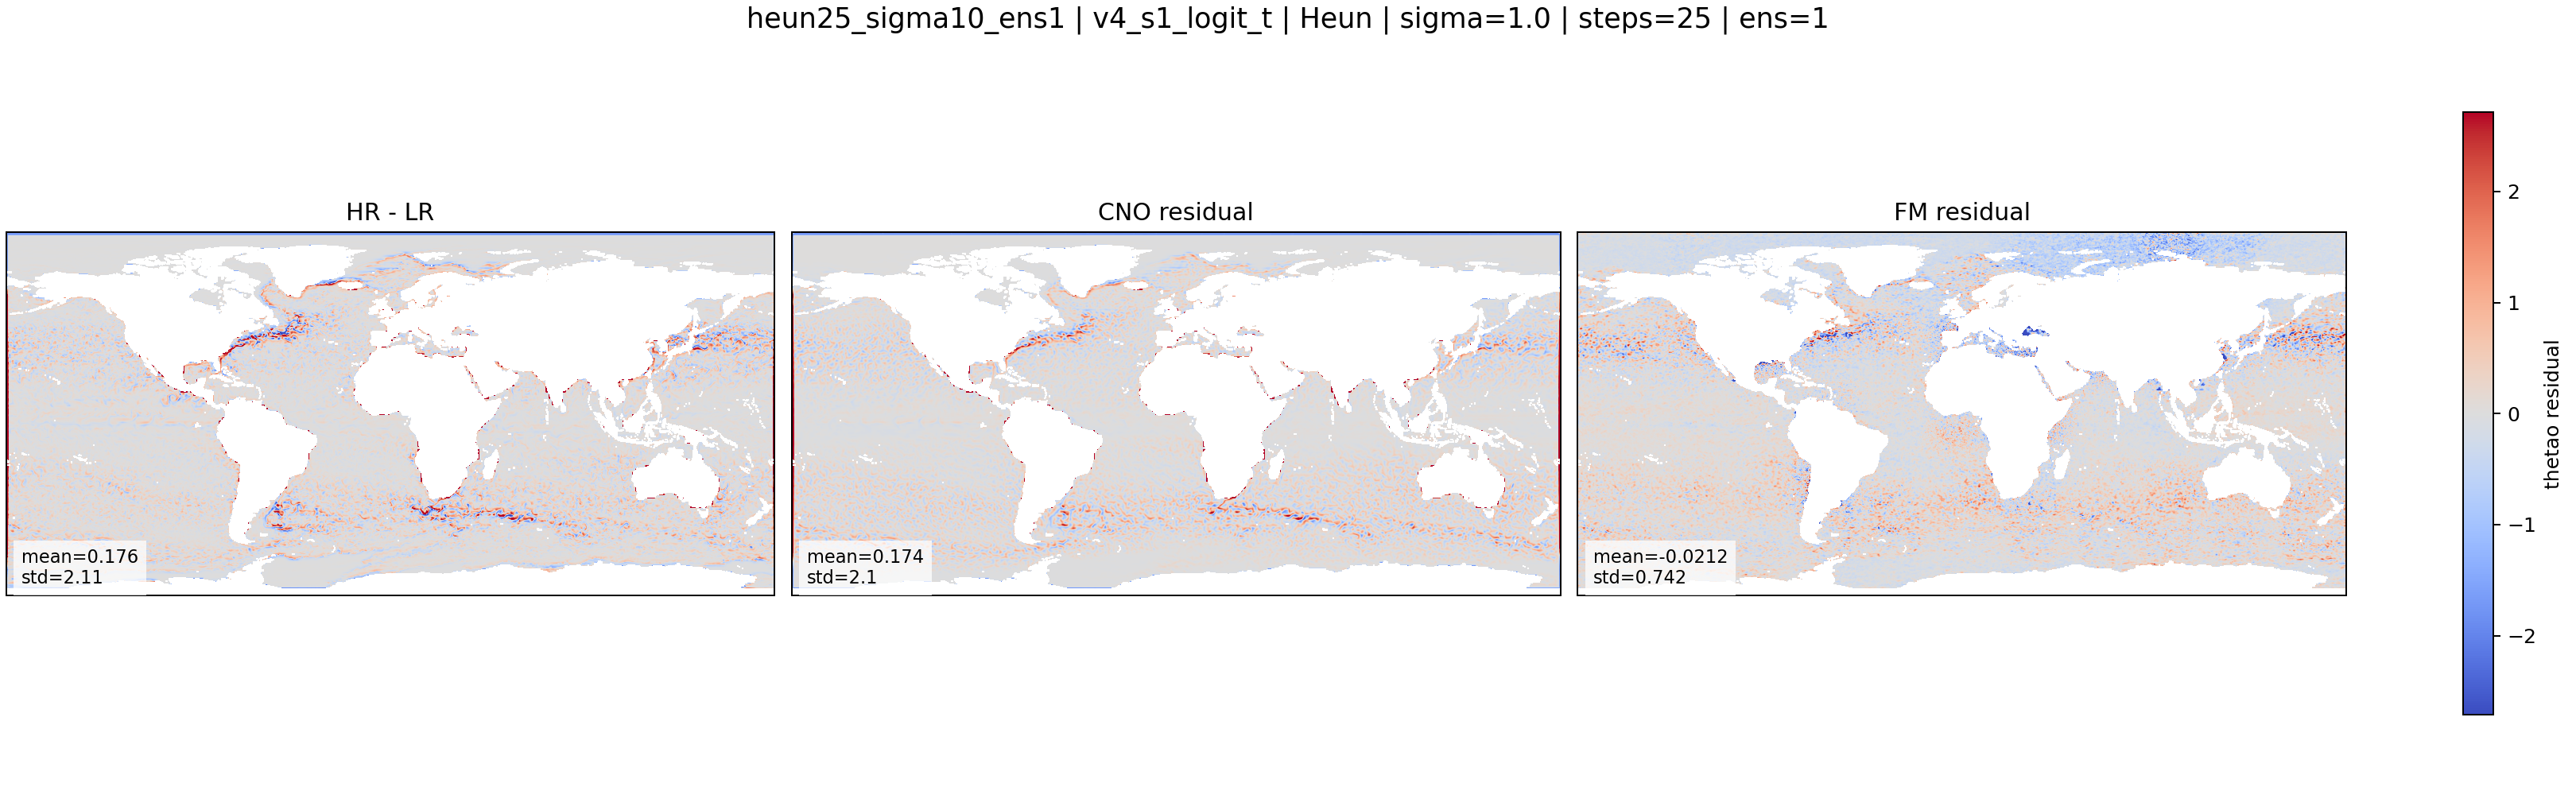
\includegraphics[width=\linewidth]{02_s1_heun25_sigma10_ens1.png}
\smallnote{Un sample: montre une réalisation.}
\column{0.49\textwidth}
\centering
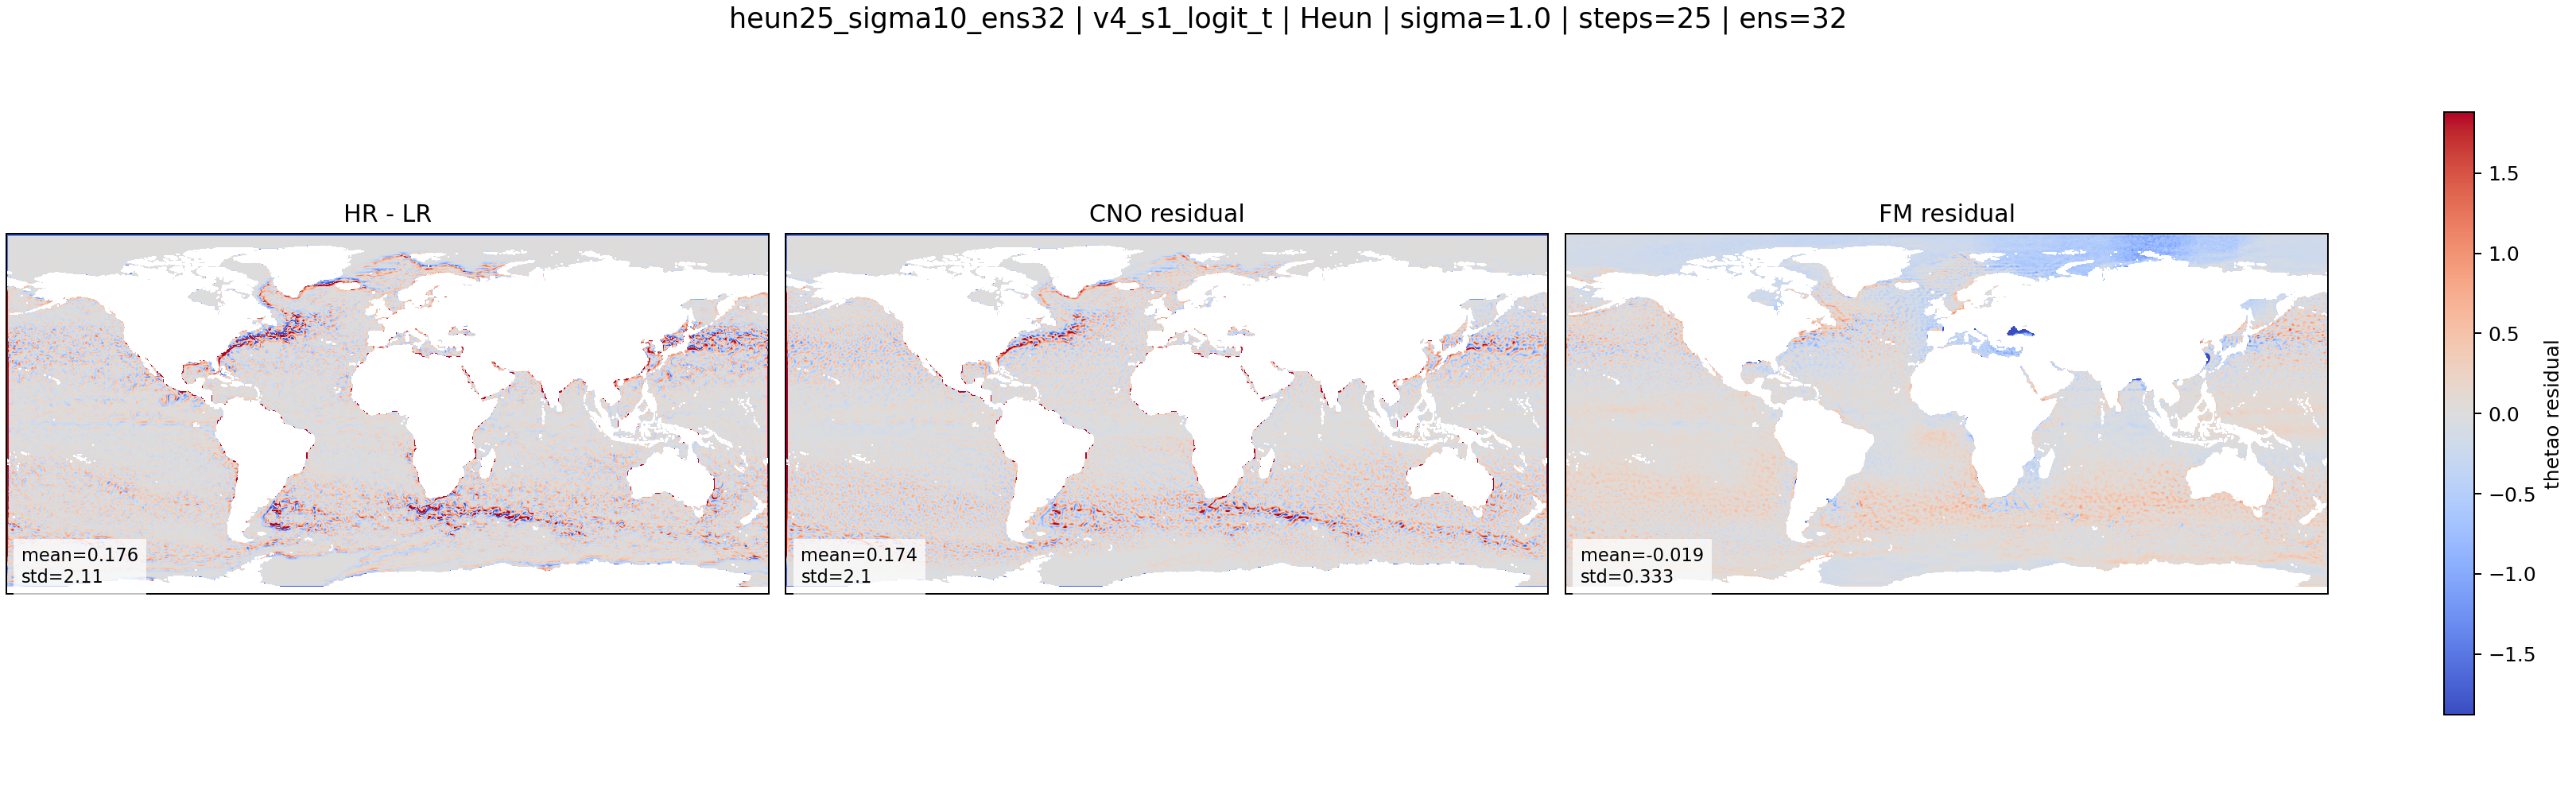
\includegraphics[width=\linewidth]{04_s1_heun25_sigma10_ens32.png}
\smallnote{Ensemble 32: moyenne/statistiques plus stables.}
\end{columns}

\vspace{0.4em}
\textbf{Lecture}: ens=32 est utile pour quantifier l'incertitude; la moyenne d'ensemble peut paraître plus lisse qu'un sample individuel.
\end{frame}

\begin{frame}{Fine-tuning 1: re-coarsening loss}
\begin{columns}[T,onlytextwidth]
\column{0.50\textwidth}
\textbf{Changement}
\begin{itemize}
  \item On part de v4\_s1\_logit\_t.
  \item On ajoute une loss de cohérence coarse/fine.
  \item On estime $\hat{x}_1 = x_t + (1-t)v_\theta$ sans intégrer l'ODE.
\end{itemize}
\textbf{Pourquoi}
\begin{itemize}
  \item Forcer la sortie HR à retrouver le LR après re-coarsening.
  \item Inspiré des pertes de consistance coarse/fine dans le downscaling récent.
\end{itemize}
\column{0.46\textwidth}
\centering
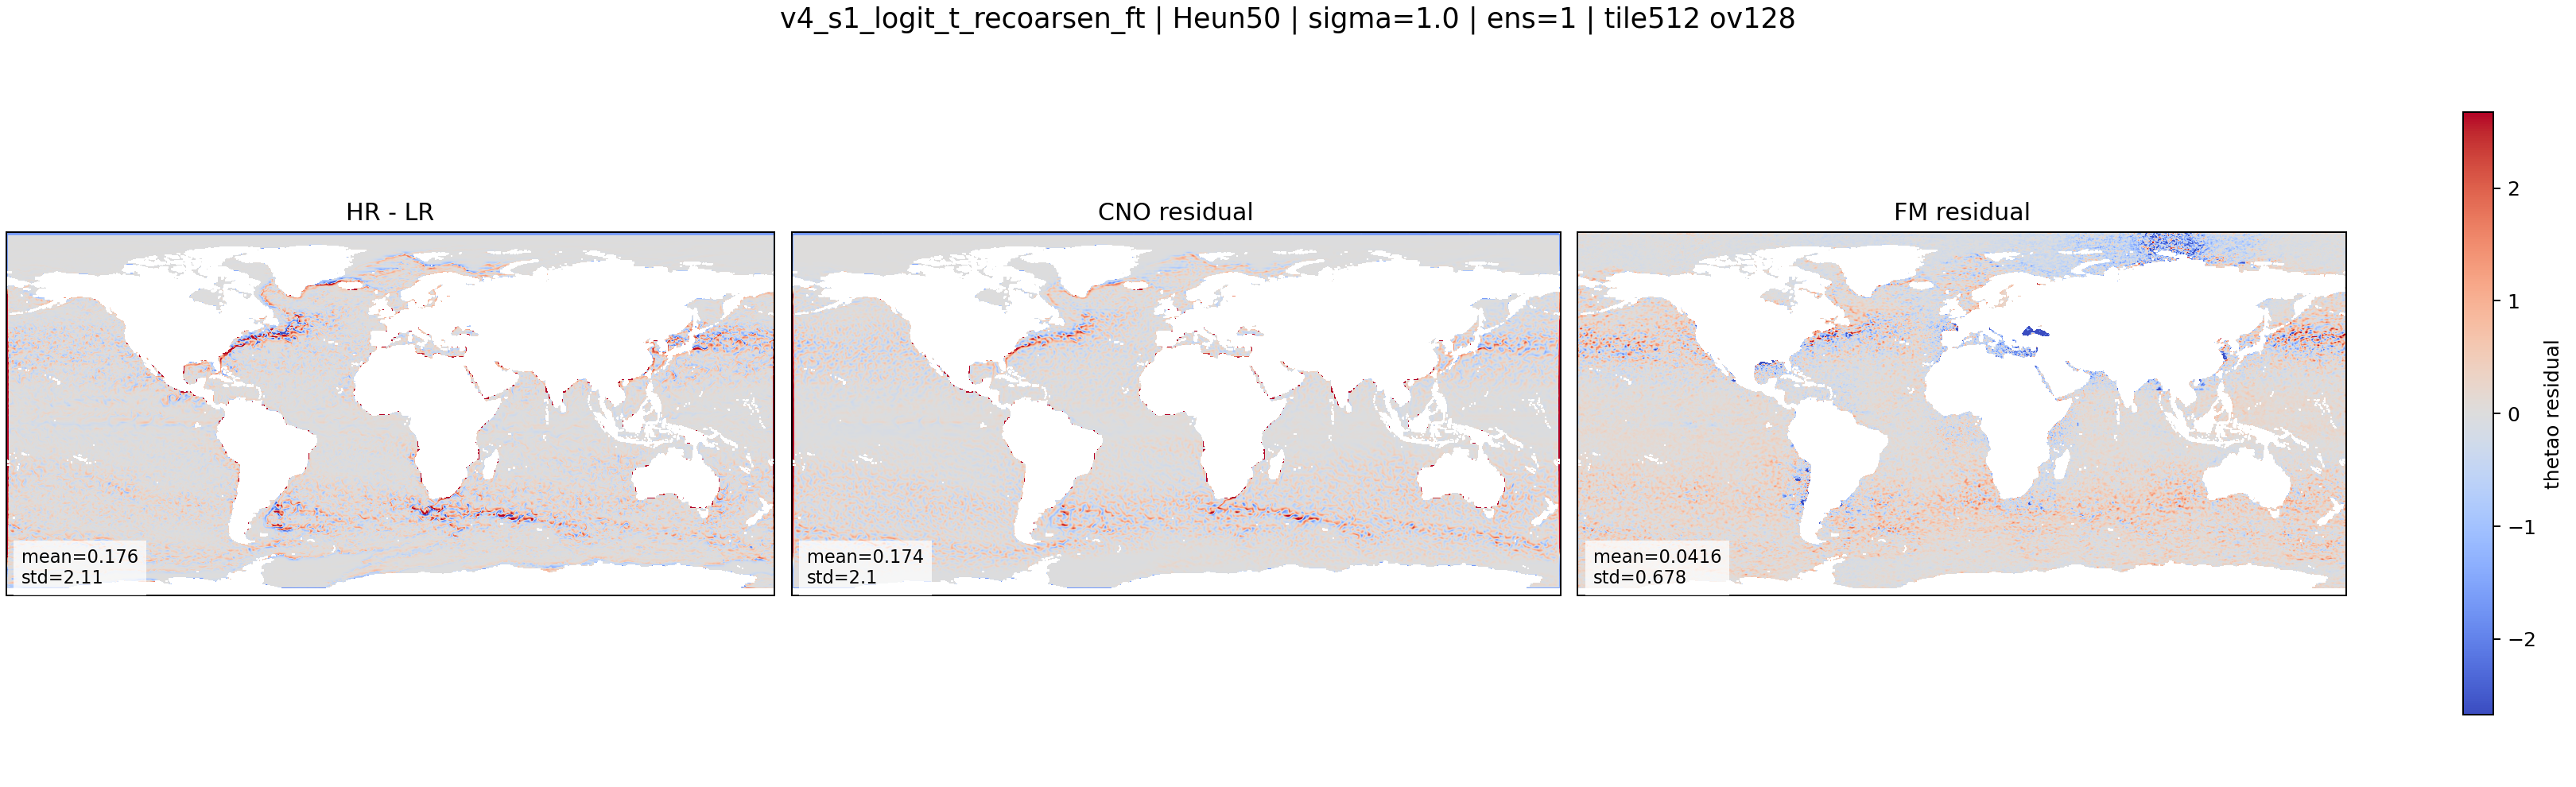
\includegraphics[width=\linewidth]{07_s1_recoarsen_ft.png}
\smallnote{Recoarsen FT, Heun 50, $\sigma=1.0$, ens=1.}
\end{columns}
\end{frame}

\begin{frame}{Fine-tuning 2: condition dropout + CFG}
\begin{columns}[T,onlytextwidth]
\column{0.52\textwidth}
\textbf{Training}
\begin{itemize}
  \item 15\% des samples ont la condition mise à zéro.
  \item Le modèle apprend deux modes: conditionné et non conditionné.
\end{itemize}
\textbf{Inférence}
\[
v_{\mathrm{guided}} = v_{\emptyset} + w(v_c - v_{\emptyset})
\]
\begin{itemize}
  \item $w=1$: normal.
  \item $w>1$: force le modèle à écouter la condition.
\end{itemize}
\column{0.44\textwidth}
\centering
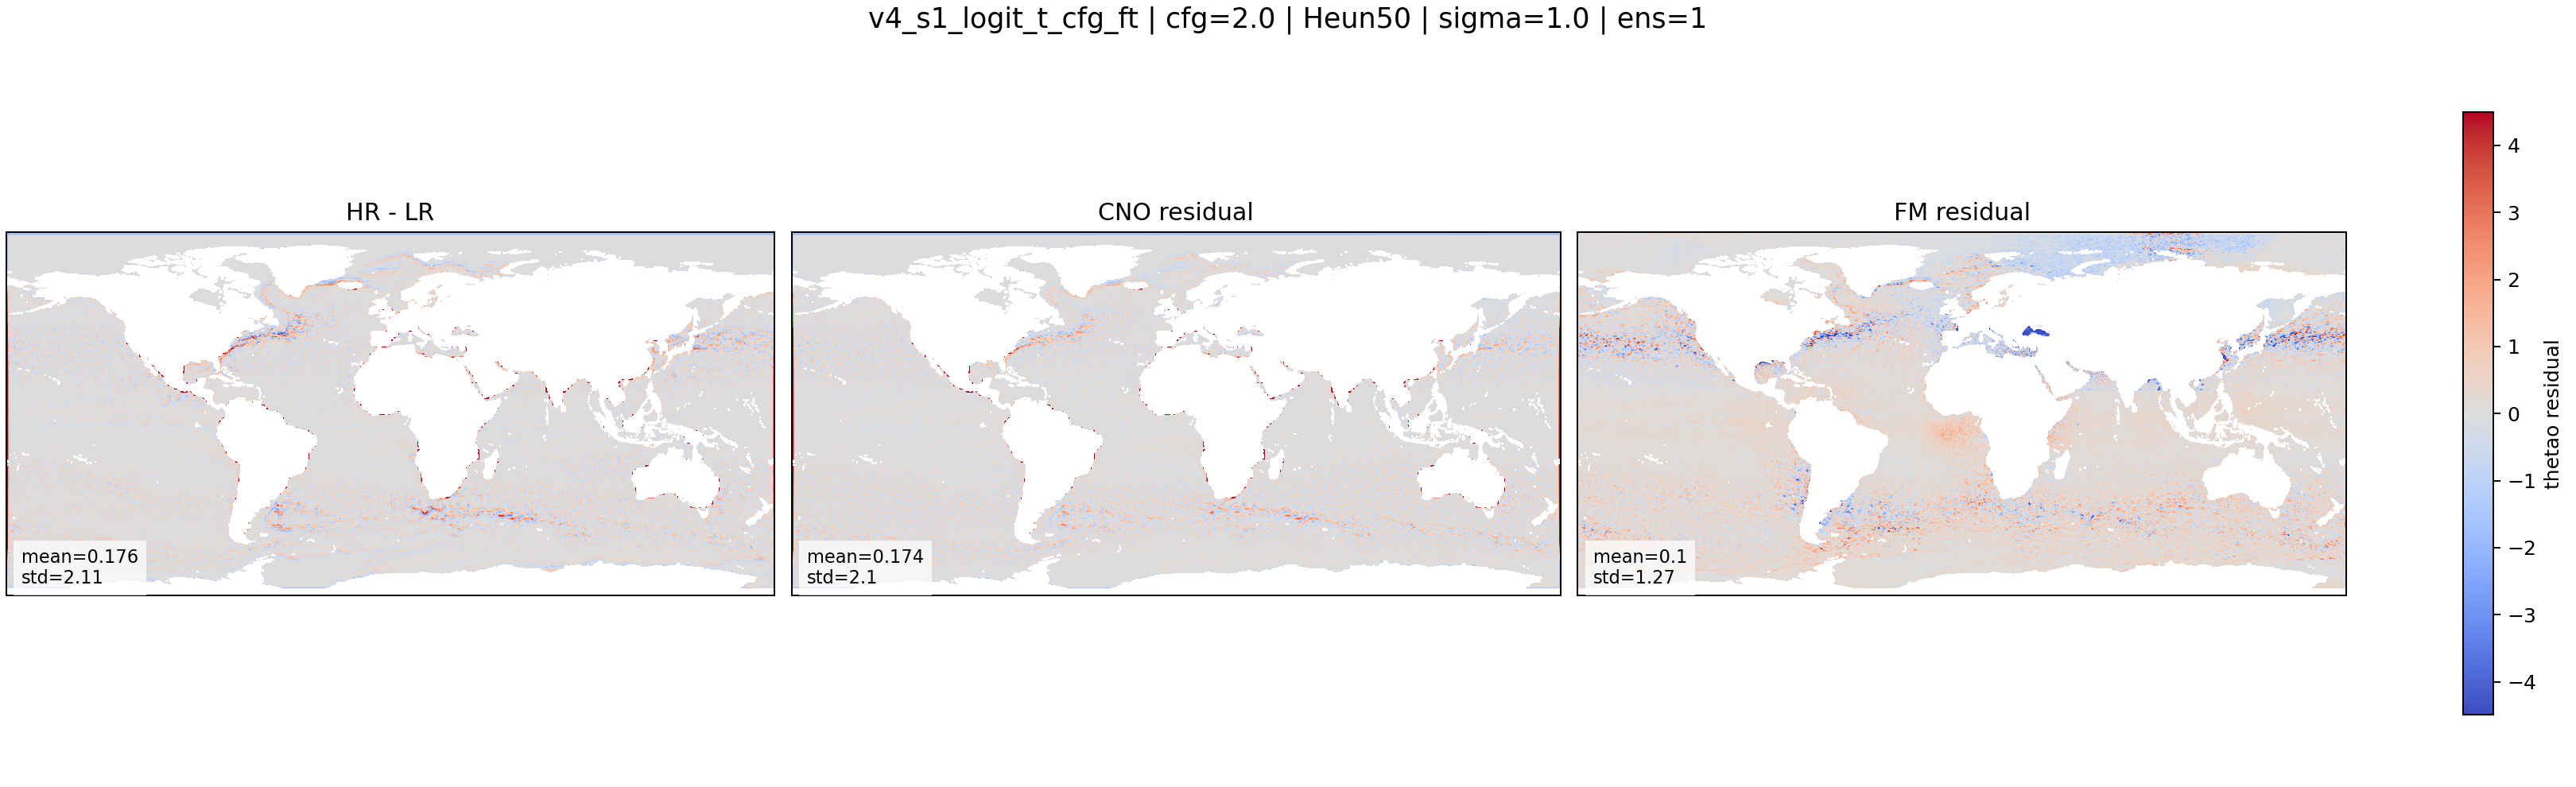
\includegraphics[width=\linewidth]{08_s1_cfg_ft_cfg2.png}
\smallnote{CFG FT, $w=2.0$, Heun 50.}
\end{columns}
\end{frame}

\begin{frame}{Sweep CFG: trop peu, correct, trop fort}
\begin{columns}[T,onlytextwidth]
\column{0.32\textwidth}
\centering
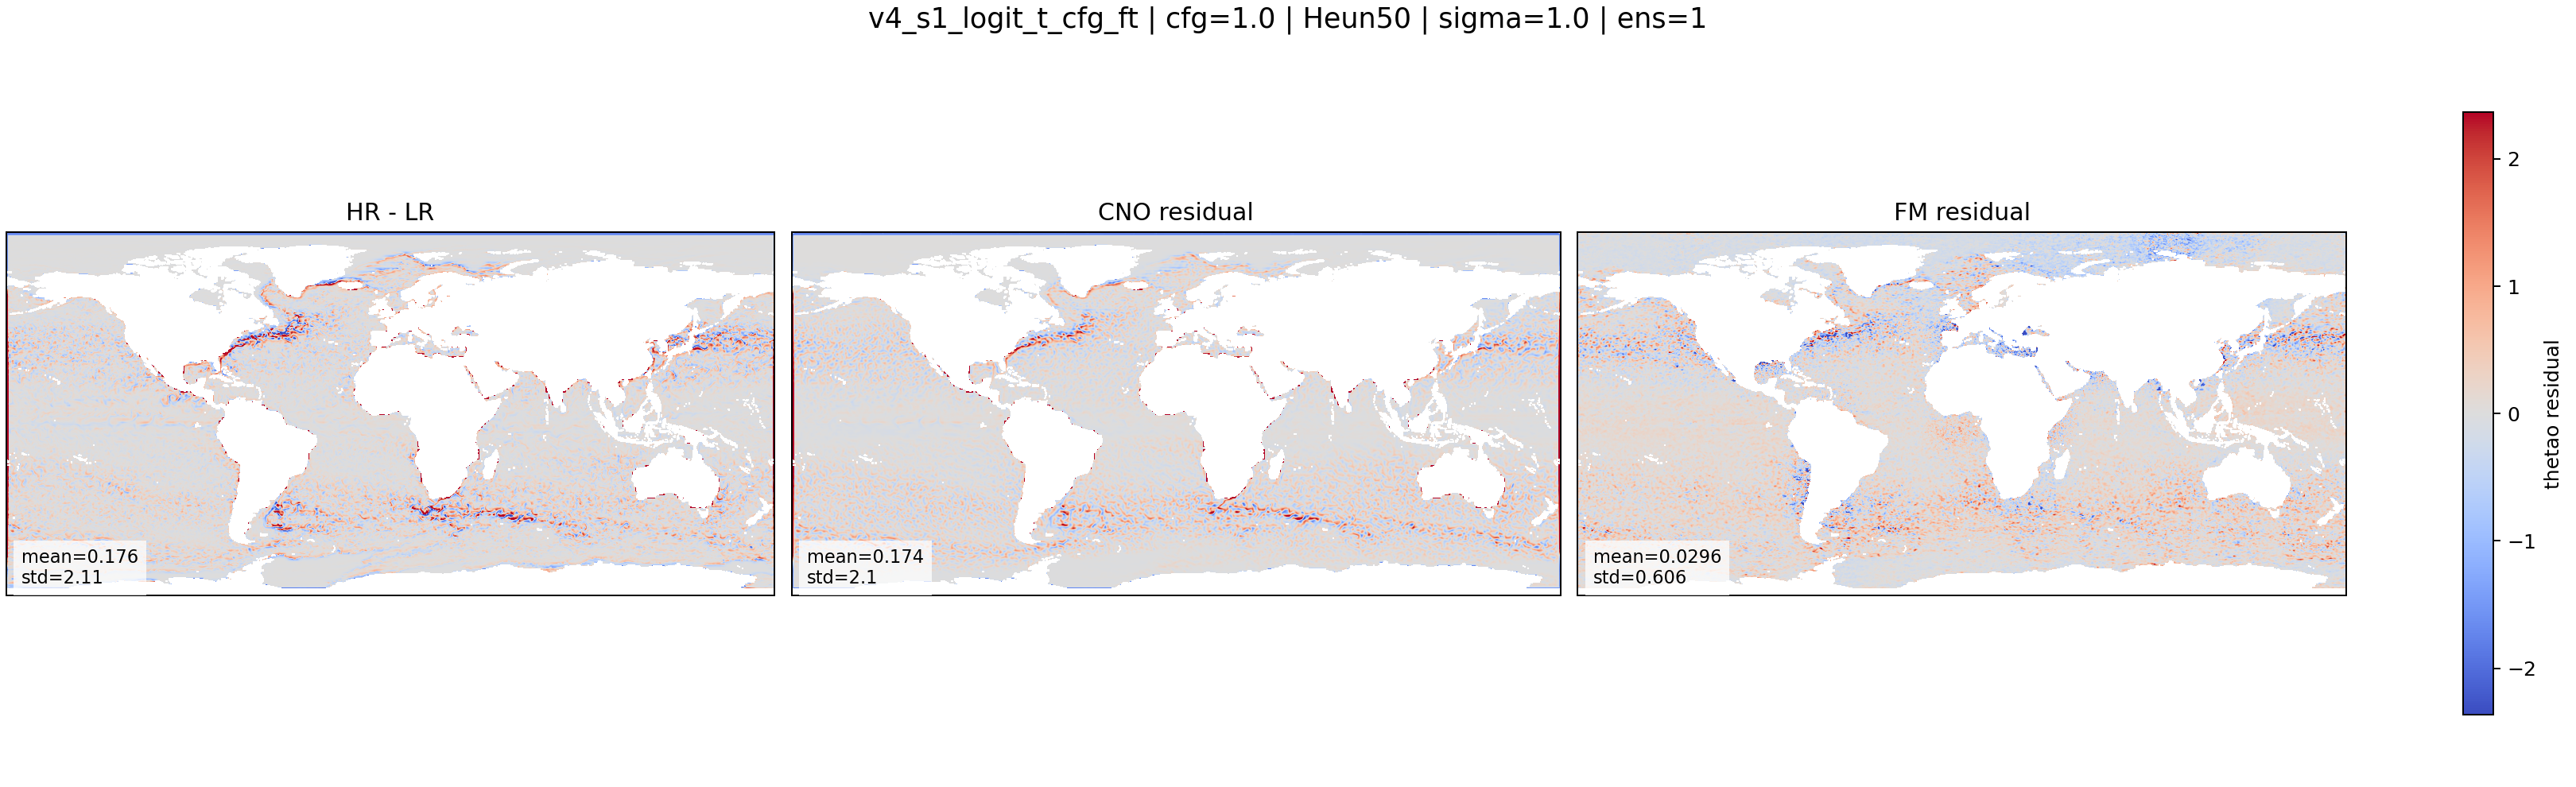
\includegraphics[width=\linewidth]{09_s1_cfg_ft_cfg1.png}
\smallnote{$w=1.0$}
\column{0.32\textwidth}
\centering
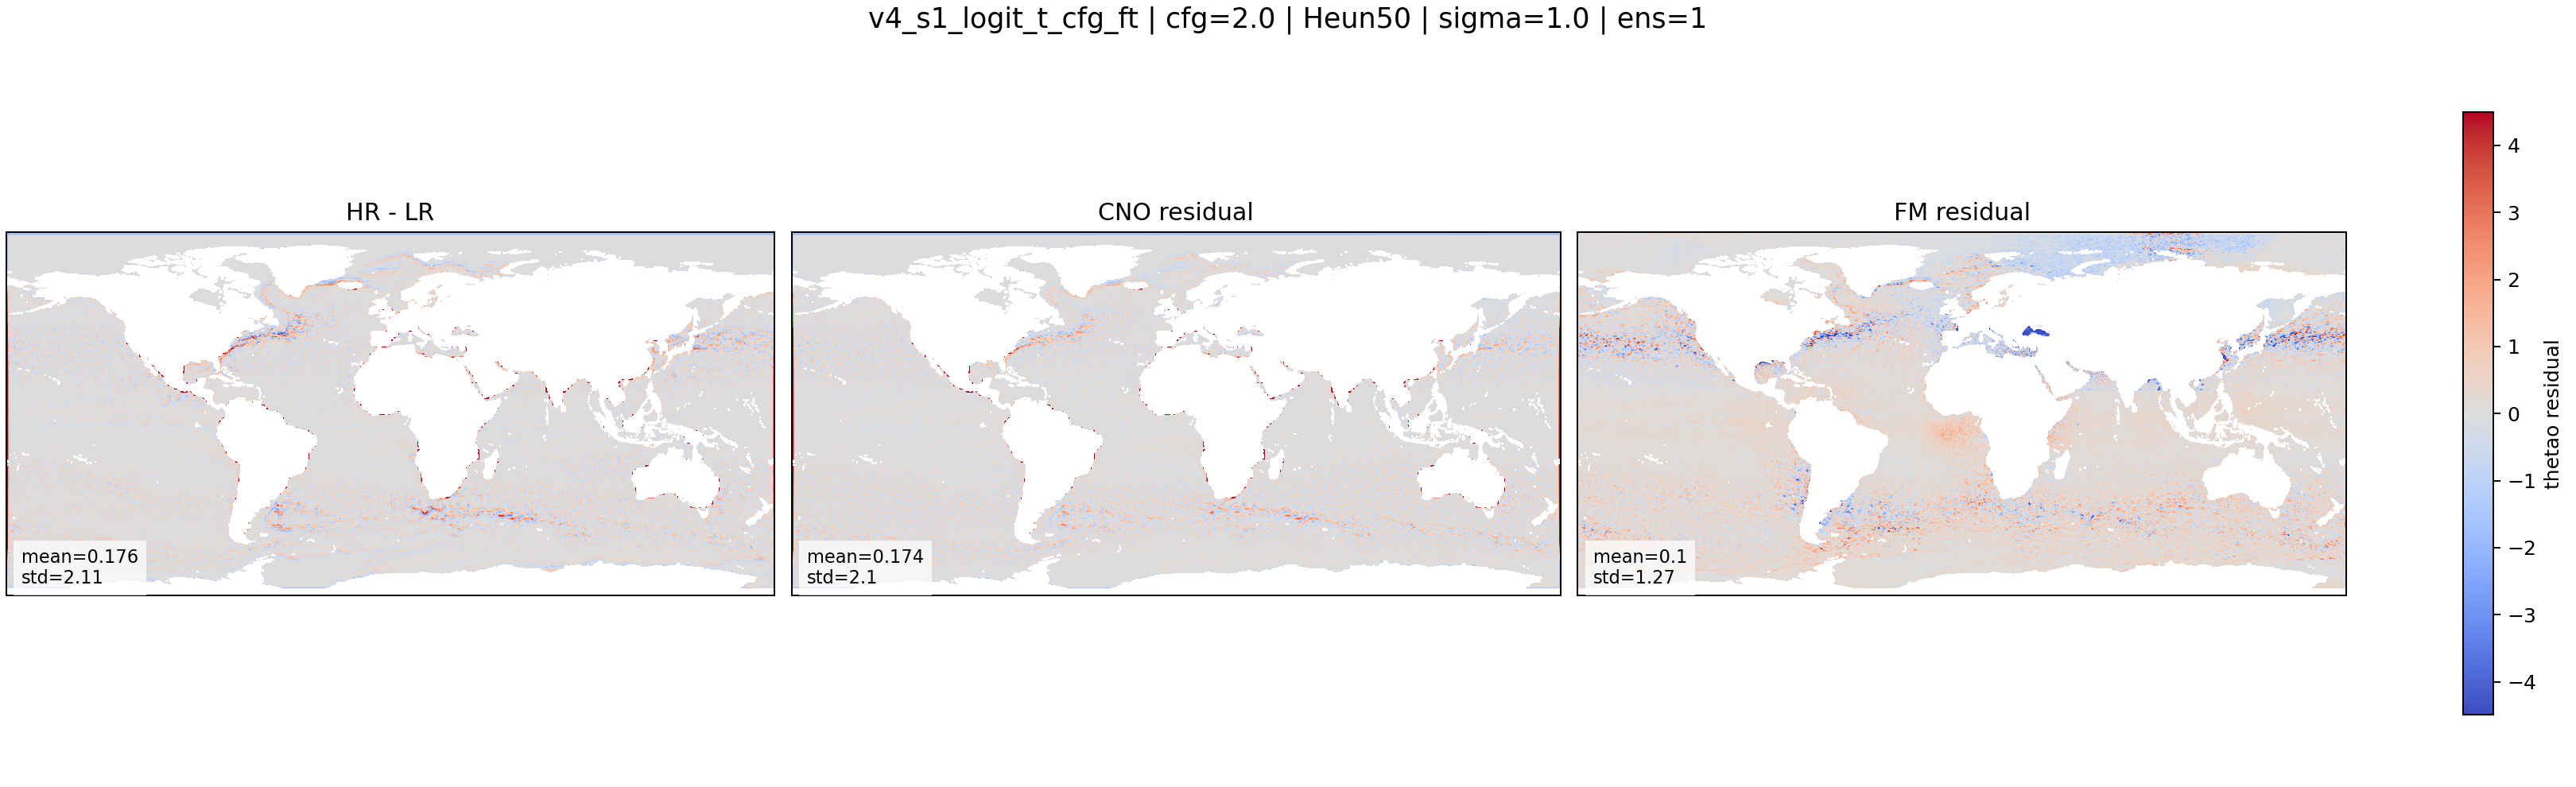
\includegraphics[width=\linewidth]{08_s1_cfg_ft_cfg2.png}
\smallnote{$w=2.0$}
\column{0.32\textwidth}
\centering
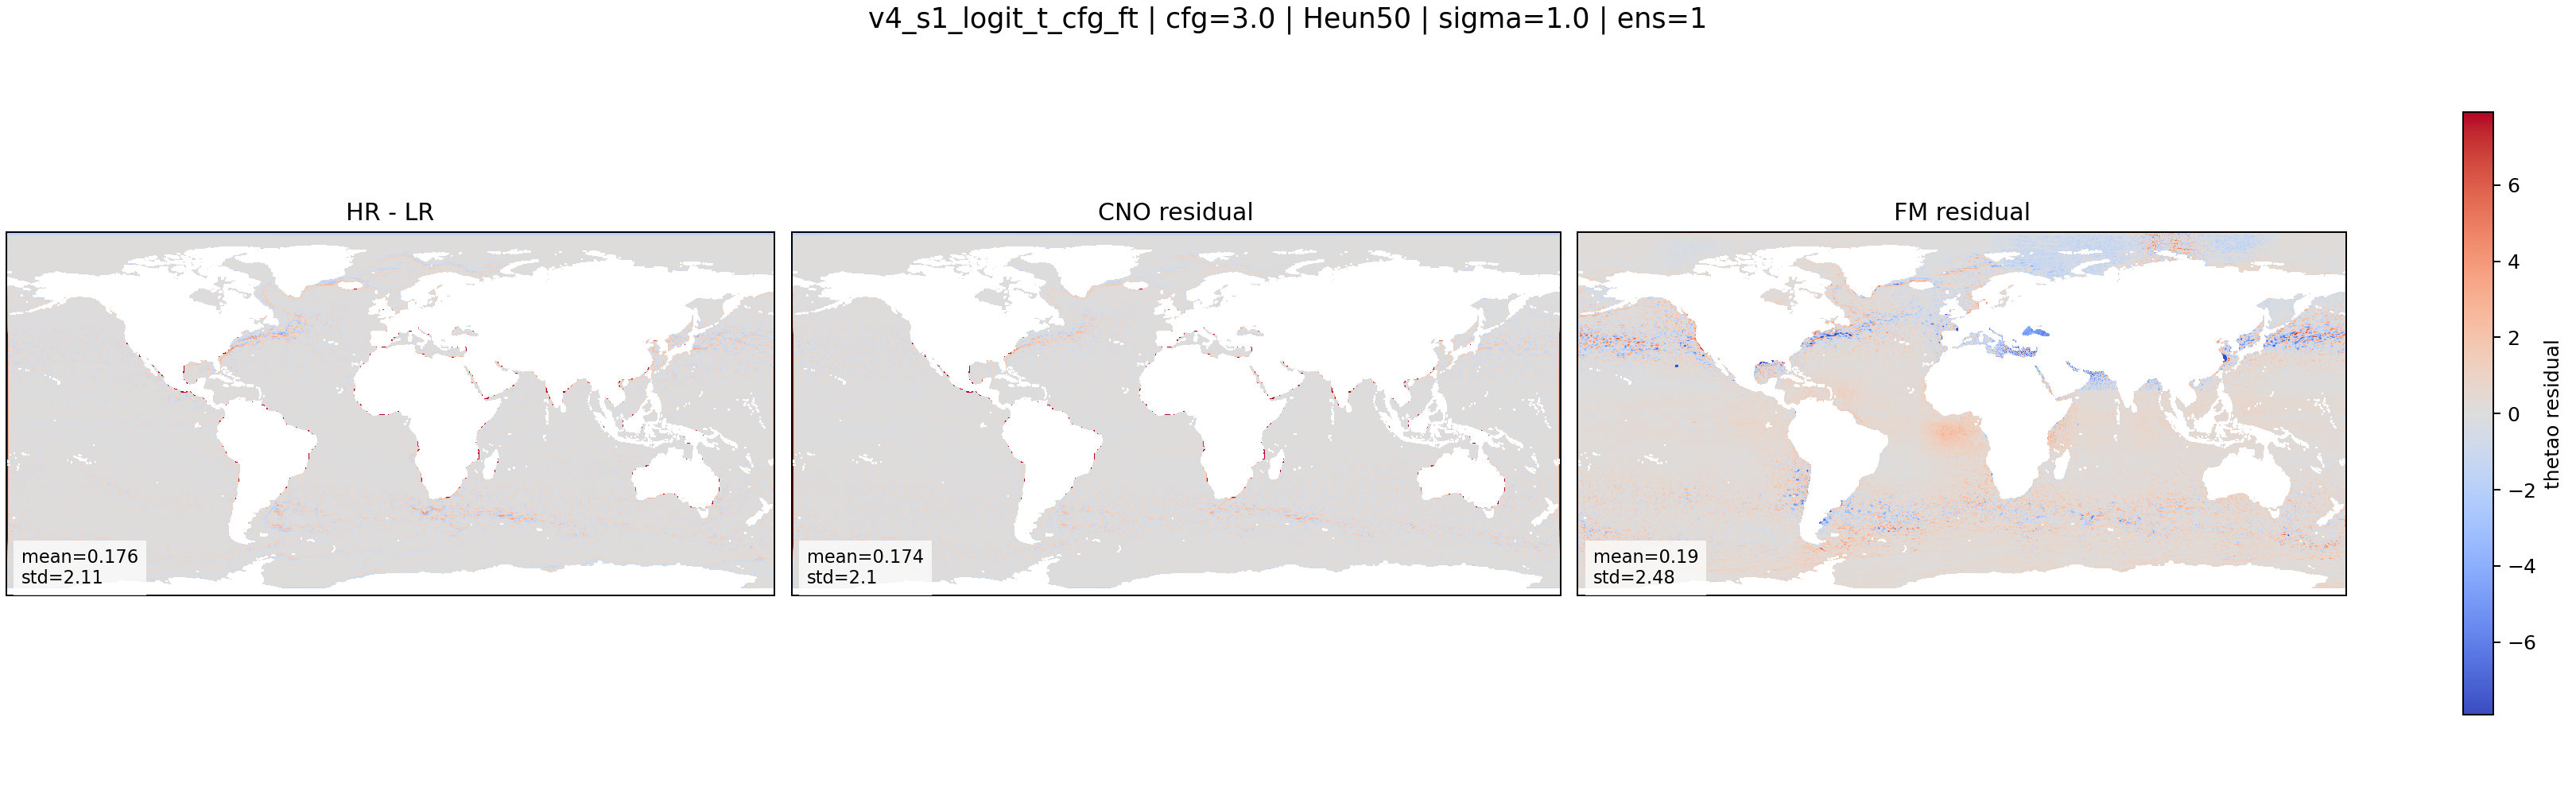
\includegraphics[width=\linewidth]{10_s1_cfg_ft_cfg3.png}
\smallnote{$w=3.0$}
\end{columns}

\vspace{0.4em}
\textbf{Interprétation}: CFG est puissant pour augmenter le contraste, mais trop haut il peut créer des sorties agressives et moins physiques.
\end{frame}

\begin{frame}{Fine-tuning 3: sampling régional}
\begin{columns}[T,onlytextwidth]
\column{0.52\textwidth}
\textbf{Problème ciblé}
\begin{itemize}
  \item Méditerranée, Mer Noire, côtes et Arctique sont sous-représentés si les patches sont tirés uniformément.
  \item Les grands bassins hauturiers dominent la distribution d'entraînement.
\end{itemize}
\textbf{Changement}
\begin{itemize}
  \item Sur-échantillonner certains patches régionaux.
  \item Objectif: corriger les erreurs régionales sans changer l'architecture.
\end{itemize}
\column{0.44\textwidth}
\centering
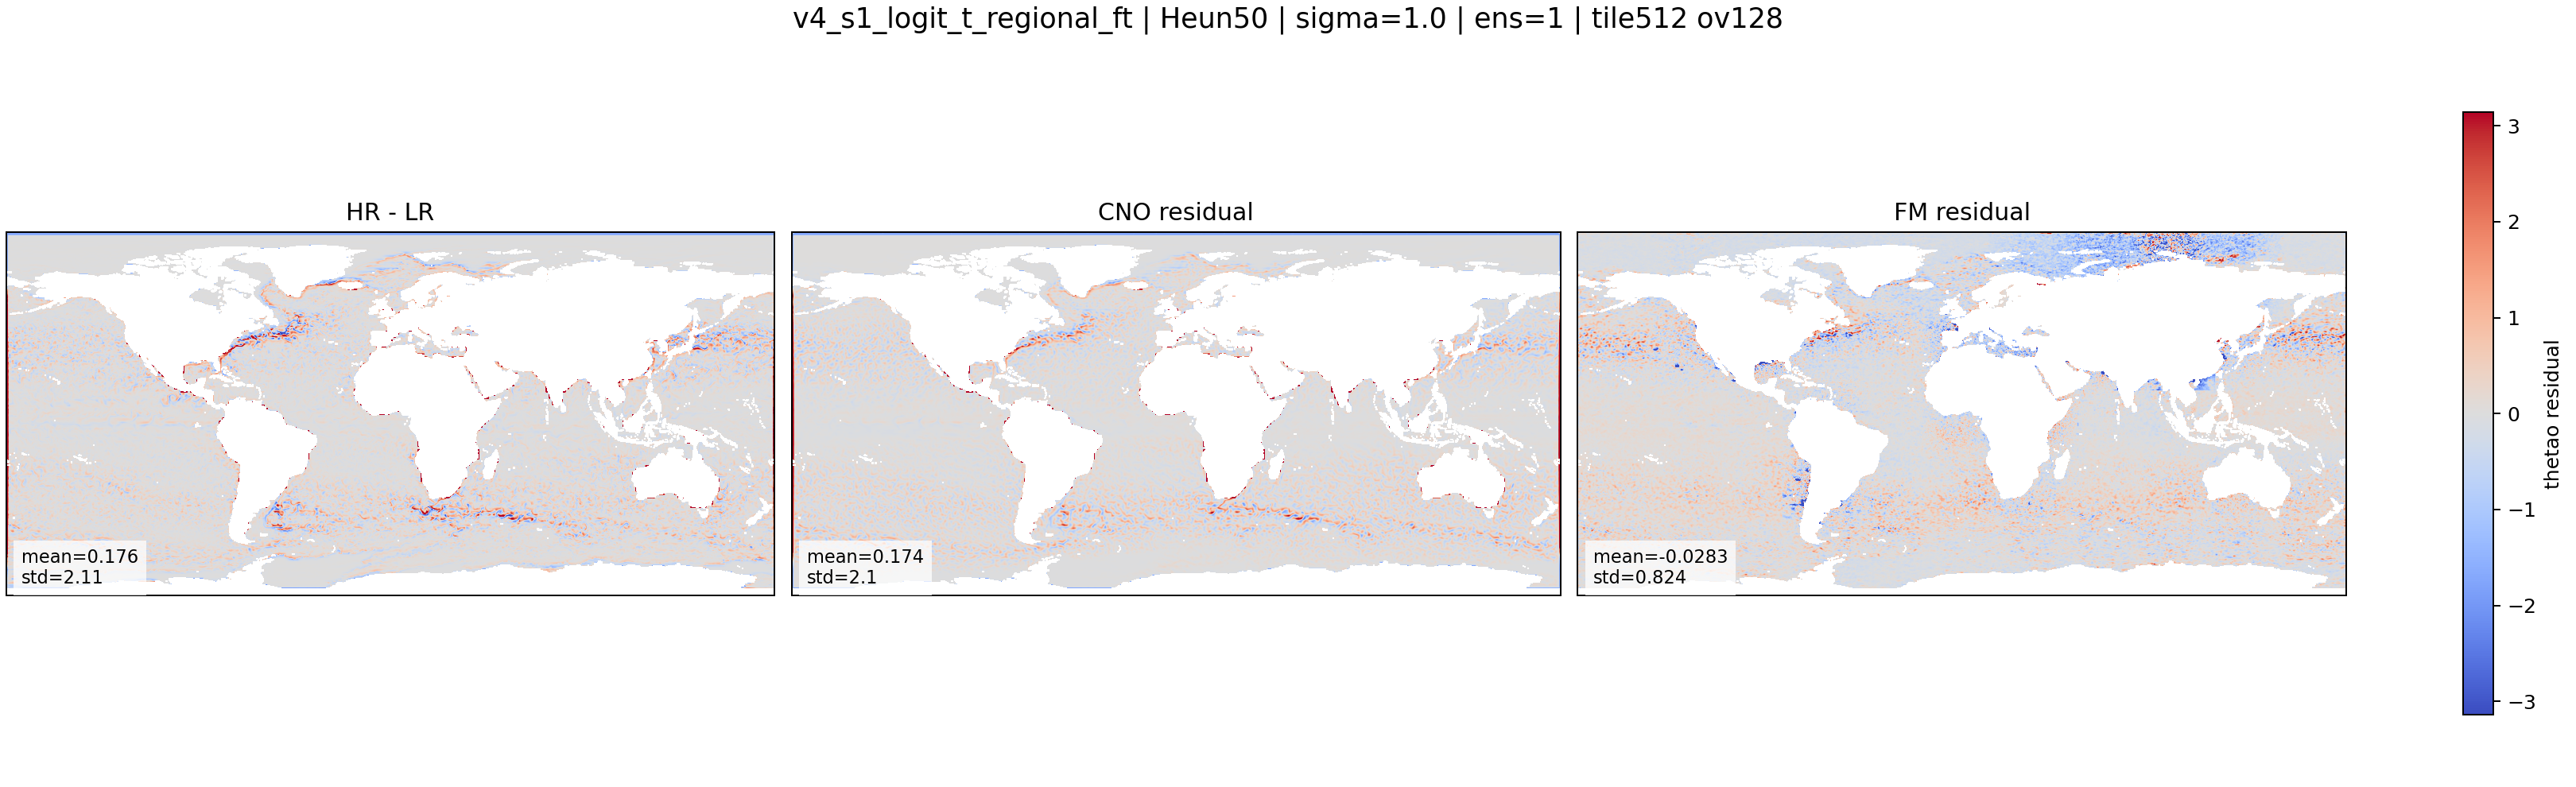
\includegraphics[width=\linewidth]{11_s1_regional_ft.png}
\smallnote{Regional FT, Heun 50, $\sigma=1.0$, ens=1.}
\end{columns}
\end{frame}

\begin{frame}{Synthèse interprétation}
\begin{table}
\scriptsize
\begin{tabular}{p{0.22\linewidth}p{0.34\linewidth}p{0.34\linewidth}}
\toprule
\textbf{Symptôme} & \textbf{Cause probable} & \textbf{Réponse testée} \\
\midrule
FM trop timide & condition CNO très forte, MSE vitesse, trajectoire prudente & logit-$t$, CFG, condition dropout \\
Artefacts côtiers & mask LR upsamplé, tuilage, distribution côtière pauvre & mask 1/12, overlap, sampling régional \\
Méditerranée / Mer Noire faibles & sous-échantillonnage régional & regional fine-tuning \\
Variance faible & modèle sous-dispersif & CFG, bruit initial, ensemble, recoarsening \\
Résultat lisse & moyenne d'ensemble / intégration stable & comparer sample vs ensemble mean \\
\bottomrule
\end{tabular}
\end{table}
\end{frame}

\begin{frame}{Ce qui est inspiré de quoi}
\begin{itemize}
  \item \textbf{Flow Matching original}: chemin $x_t$, apprentissage d'un champ de vitesse.
  \item \textbf{Conditional Flow Matching / OT}: idée de coupling entre bruit et cible, minibatch-OT.
  \item \textbf{Diffusion / EDM / FM récents}: logit-normal $t$, bruit initial, CFG.
  \item \textbf{CorrDiff / AFM / PC-AFM}: solveurs plus robustes, contraintes coarse/fine, downscaling conditionnel.
  \item \textbf{Delefosse et downscaling météo FM}: re-coarsening consistency pour imposer que HR redonne LR.
\end{itemize}
\smallnote{Les références exactes peuvent être ajoutées en backup avec les arXiv si besoin.}
\end{frame}

\begin{frame}{Conclusion opérationnelle}
\begin{itemize}
  \item \textbf{Base à présenter}: v4\_s1\_logit\_t.
  \item \textbf{Meilleur test inference rapide}: Heun 50, $\sigma=1.0$, ens=1.
  \item \textbf{Test variance}: condition dropout + CFG sweep.
  \item \textbf{Test physique}: re-coarsening loss, sans Laplacien au début.
  \item \textbf{Test régional}: sampling pondéré Med/Mer Noire/Arctique.
  \item \textbf{Pour la démo Edito}: impératif d'utiliser le mask océan 1/12 pour les sorties.
\end{itemize}
\end{frame}

\begin{frame}{Backup: CFG ensemble}
\centering
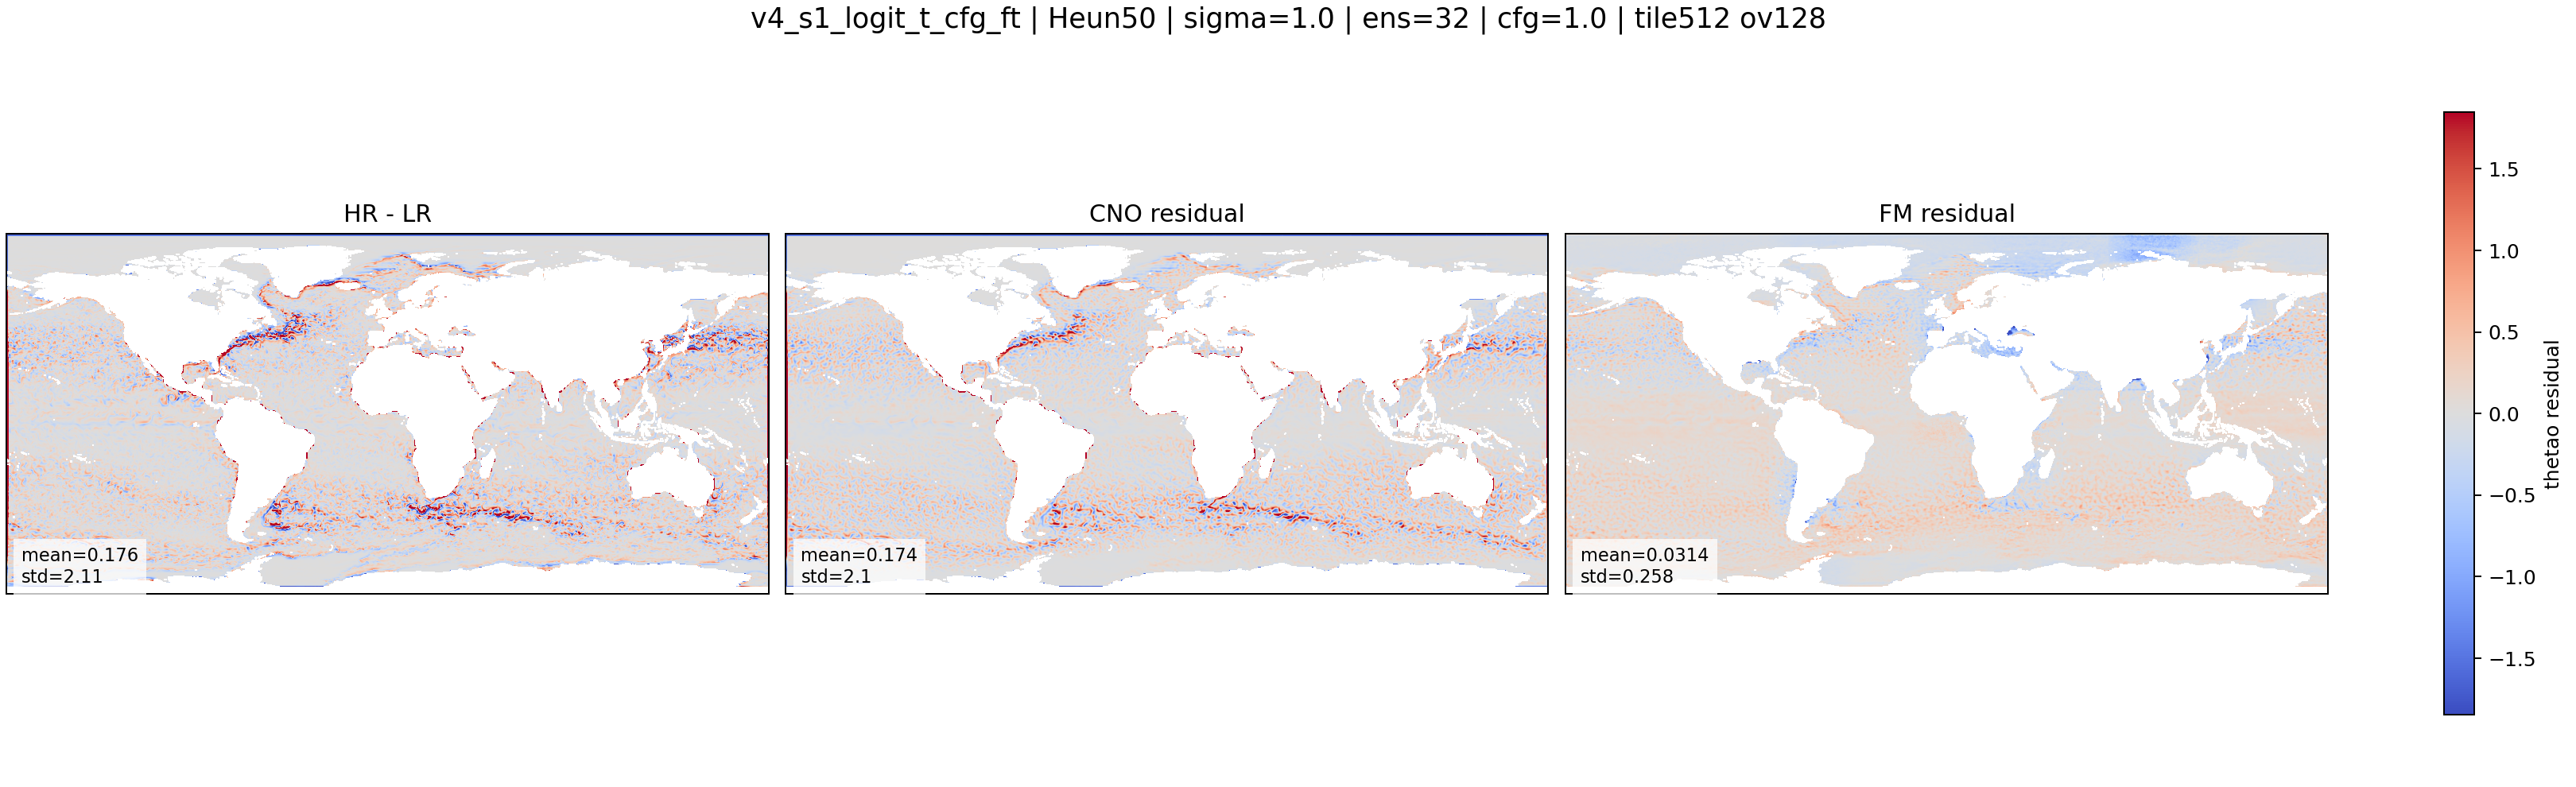
\includegraphics[width=0.85\linewidth,height=0.76\textheight,keepaspectratio]{12_s1_cfg_ft_ens32_cfg1.png}
\smallnote{CFG FT, ens=32. À lire comme incertitude/moyenne, pas comme sample unique.}
\end{frame}

\end{document}
